\documentclass[a4paper,UKenglish]{lipics-v2016}
%This is a template for producing LIPIcs articles. 
%See lipics-manual.pdf for further information.
%for A4 paper format use option "a4paper", for US-letter use option "letterpaper"
%for british hyphenation rules use option "UKenglish", for american hyphenation rules use option "USenglish"
% for section-numbered lemmas etc., use "numberwithinsect"
 
\usepackage{microtype}%if unwanted, comment out or use option "draft"

%\graphicspath{{./graphics/}}%helpful if your graphic files are in another directory

\bibliographystyle{plainurl}% the recommended bibstyle

% Author macros::begin %%%%%%%%%%%%%%%%%%%%%%%%%%%%%%%%%%%%%%%%%%%%%%%%
\title{\jilette: Symbolic Execution for JavaScript}
\titlerunning{\jilette: Symbolic Execution for JavaScript} %optional, in case that the title is too long; the running title should fit into the top page column

%% Please provide for each author the \author and \affil macro, even when authors have the same affiliation, i.e. for each author there needs to be the  \author and \affil macros
\author[1]{Anonymous Authors}
%\affil[1]{Anonymous Affiliation}

%\affil[1]{ University Computing Laboratory, Address/City, Country\\
%  \texttt{open@dummyuniversity.org}}
%\authorrunning{Anonymous authors} %mandatory. First: Use abbreviated first/middle names. Second (only in severe cases): Use first author plus 'et. al.'

\Copyright{Anonymous Authors}%mandatory, please use full first names. LIPIcs license is "CC-BY";  http://creativecommons.org/licenses/by/3.0/

%\subjclass{Classification}% mandatory: Please choose ACM 1998 classifications from http://www.acm.org/about/class/ccs98-html . E.g., cite as "F.1.1 Models of Computation". 
%\keywords{}% mandatory: Please provide 1-5 keywords
% Author macros::end %%%%%%%%%%%%%%%%%%%%%%%%%%%%%%%%%%%%%%%%%%%%%%%%%

%Editor-only macros:: begin (do not touch as author)%%%%%%%%%%%%%%%%%%%%%%%%%%%%%%%%%%
\EventEditors{Editor E. Editor}
\EventNoEds{1}
\EventLongTitle{32nd European Conference on Object-Oriented Programming (ECOOP)}
\EventShortTitle{ECOOP 2018}
\EventAcronym{ECOOP}
\EventYear{2018}
\EventDate{July 16--22, 2018}
\EventLocation{Amsterdam, The Netherlands}
\EventLogo{}
%\SeriesVolume{42}
%\ArticleNo{23}
% Editor-only macros::end %%%%%%%%%%%%%%%%%%%%%%%%%%%%%%%%%%%%%%%%%%%%%%%

%External Packages
%\usepackage{amsthm}
%\usepackage[utf8x]{inputenc}
\usepackage[table]{xcolor}
\usepackage{amsmath}
\usepackage{listings}
\usepackage{hyperref}
\usepackage{graphicx}
\usepackage{tabularx}
\usepackage{xspace}
\usepackage{textcomp}
\usepackage{amssymb,amsfonts,latexsym,wasysym,mathrsfs,textcomp,stmaryrd}
\usepackage{mathpartir}
\usepackage{url}
\usepackage{upgreek}
\usepackage{xparse}
\usepackage{booktabs}
%\usepackage{stix}

%\usepackage{algorithm}
%\usepackage{algpseudocode}

\usepackage{wrapfig}

%JavaScript 
\definecolor{SkyBlue}{rgb}{0.20,0.39,0.64}
\definecolor{Plum}{rgb}{0.46,0.31,0.48}
\definecolor{Chocolate}{rgb}{0.75,0.49,0.07}
\definecolor{Aluminium5}{rgb}{0.33,0.34,0.32}
\definecolor{DarkGreen}{rgb}{0.2,0.5,0.2}
\definecolor{ltblue}{rgb}{0,0.4,0.4}
\definecolor{dkblue}{rgb}{0,0.2,0.7}
\definecolor{dkgreen}{rgb}{0,0.4,0}
\definecolor{dkviolet}{rgb}{0.3,0,0.5}
\definecolor{dkred}{rgb}{0.6,0,0}
\definecolor{talkred}{rgb}{0.69,.20,0.22}
\definecolor{talkblue}{rgb}{0.04,0.40,0.80}
\definecolor{talkgreen}{rgb}{0.34,.81,0.10}
\definecolor{oldtalkblue}{rgb}{0.22,.20,0.69}
\definecolor{greenish}{rgb}{.0,.65,.0}
\definecolor{mygray}{gray}{0.9}

\lstdefinelanguage{JavaScript}{
  morekeywords=[1]{typeof, new, true, false, catch,
    function, return, null, catch, switch, var,
    if, in, while, do, else, case, break, continue},
  morekeywords=[2]{class, export, boolean, throw, implements, import, this},
  numbers=left,
  numbersep=4pt,
  numberstyle=\tiny\color{dkblue},
  columns=fullflexible,
  sensitive=false,
  comment=[l]{//},
  captionpos=b,   
  morecomment=[s]{/*}{*/},
  morestring=[b]',
  morestring=[b]",
  basicstyle=\scriptsize\texttt,
  identifierstyle=\ttfamily\color{Aluminium5},
  keywordstyle=[1]\ttfamily\color{Plum},
  keywordstyle=[2]\ttfamily\color{SkyBlue},
  stringstyle=\ttfamily\color{DarkGreen},
  commentstyle=\ttfamily, 
%  commandchars=\$\{\}
}[keywords,comments,strings]

\lstdefinelanguage{Scheme}{
  morekeywords=[1]{define, define-syntax, define-macro, lambda, define-stream, stream-lambda},
  morekeywords=[2]{begin, call-with-current-continuation, call/cc,
    call-with-input-file, call-with-output-file, case, cond,
    do, else, for-each, if,
    let*, let, let-syntax, letrec, letrec-syntax,
    let-values, let*-values,
    and, or, not, delay, force,
    quasiquote, quote, unquote, unquote-splicing,
    map, fold, syntax, syntax-rules, eval, environment, query },
  morekeywords=[3]{import, export},
  alsodigit=!\$\%&*+-./:<=>?@^_~,
  sensitive=true,
  morecomment=[l]{;},
  morecomment=[s]{\#|}{|\#},
  morestring=[b]",
  basicstyle=\scriptsize\ttfamily,
  keywordstyle=\bf\ttfamily\color[rgb]{0,.3,.7},
  commentstyle=\color[rgb]{0.133,0.545,0.133},
  stringstyle={\color[rgb]{0.75,0.49,0.07}},
  upquote=true,
  breaklines=true,
  breakatwhitespace=true,
  literate=*{`}{{`}}{1}
}

\def\schemeinline{\lstinline[language=Scheme, basicstyle=\small\ttfamily]}

\lstnewenvironment{lstjs}{\lstset{language=JavaScript,basicstyle=\fontsize{8}{8}\ttfamily,escapeinside={~}{~}}}{}
\def\jsinline{\lstinline[language=JavaScript, basicstyle=\small]}


% The Acronyms of the project and some other stuff
\newcommand{\jsil}{JSIL\xspace}
\newcommand{\jsverify}{JSVerify\xspace}
\newcommand{\JSComp}{JS-2-JSIL\xspace}
\newcommand{\jsilverify}{JSILVerify\xspace}


% Tikz 
\usepackage{tikz}
\usetikzlibrary{calc,positioning,arrows,shapes,decorations.pathmorphing}
\usetikzlibrary{arrows,positioning} 
\tikzset{
    %Define standard arrow tip
    >=stealth',
    % Define arrow style
    pil/.style={
           ->,
           shorten <=2pt,
           shorten >=2pt,}
}

\newcommand{\runpic}{\includegraphics[width=0.06\picwidth]{running.pdf}}
\newcommand{\tickpic}{\resizebox{0.06\picwidth}{!}{\(\color{greenish} \checkmark \)}}
\tikzset{
  box/.style = {rectangle, draw=black,align=center,font=\scriptsize},
  sbox/.style = {rectangle,draw=black,align=left,font=\scriptsize,text width=1.7cm},
  p/.style = {-latex},
  dp/.style = {latex-latex},
  sz/.style n args={2}{minimum width=#2, minimum height=#1},
  m/.style = {midway,inner sep=0pt,fill=white},
  ll/.style = {font=\scriptsize,anchor=south west}
}



% Polishing...
\newcommand{\polish}[1]{{\color{red}#1}}

% macros_js as for Jose Santos
\usepackage{macros_js}
\usepackage{gdshojs}

\newcommand{\jilette}{Cosette\xspace}
\newcommand{\rosette}{Rosette\xspace}

\newcommand{\myparagraph}[1]{\smallskip\noindent {\bf #1.}\hspace{1pt}}
\newcommand{\myparagraphq}[1]{\smallskip\noindent {\bf #1?}\hspace{1pt}}

% COMMENTS

\newcommand{\pginline}[1]{ {\color{red} *** PG : #1 ***} }
\newcommand{\pmaxinline}[1]{ {\color{blue} *** PM : #1 ***} }
\newcommand{\jfsinline}[1]{ {\color{green} *** JFS : #1 ***} }
\newcommand{\jdinline}[1]{ {\color{purple} *** JD : #1 ***} }

\newif\ifComments
\Commentstrue

\newcommand{\pg}[1]{%
\ifComments
\begin{center}
\fbox{\begin{minipage}{0.95\textwidth} \color{red}
{\rm PG: \small #1}
\end{minipage}}
\end{center}
\fi}

\newcommand{\pmax}[1]{%
\ifComments
\begin{center}
\fbox{\begin{minipage}{0.95\textwidth} \color{blue}
{\rm PM: \small #1}
\end{minipage}}
\end{center}
\fi}

\newcommand{\jfs}[1]{%
\ifComments
\begin{center}
\fbox{\begin{minipage}{0.95\textwidth} \color{green}
{\rm JFS: \small #1}
\end{minipage}}
\end{center}
\fi}

\newcommand{\jd}[1]{%
\ifComments
\begin{center}
\fbox{\begin{minipage}{0.95\textwidth} \color{purple}
{\rm JD: \small #1}
\end{minipage}}
\end{center}
\fi}

%



\begin{document}
%

\maketitle 

\begin{abstract}
We present \jilette, a symbolic execution tool for JavaScript (ECMAScript 5, ES5), which precisely follows the language standard. At the core of \jilette is a sound symbolic interpreter for \jsil, an intermediate language well-suited for verification and analysis. This interpreter is written in \underline{Rosette}, %~\cite{Rosette2,Rosette1}, 
a symbolic virtual machine that enables the design of new solver-aided languages. 
\jilette works by first compiling JavaScript programs to \jsil using \underline{\JSComp}, %~\cite{javert}, 
a well-tested, standard-compliant compiler from JavaScript to \jsil, and then symbolically executing the compiled \jsil code in the \jsil symbolic interpreter. 
We study two complementary uses of \jilette. 
First, we show how \jilette can be used for symbolic testing of JavaScript programs by finding concrete executions that trigger assertion and test failures. 
We highlight the range of \jilette by giving examples using strings, regular expressions, and the notorious \jsinline|eval| statement.
Second, building on \jilette, we develop a tool for debugging separation logic specifications by compiling them to symbolic tests in order to find 
witnesses for bugs in both specification and code.
\vspace*{-0.4cm}
\end{abstract}

\section{Introduction}

\vspace*{-0.2cm}
JavaScript is the most widespread dynamic language: it is the de facto language for client-side Web applications (used by 94.8\% of websites \cite{JS948percent});
it is used for server-side scripting via Node.js; and it is even run on small embedded devices with limited 
memory. It is the most active language in both GitHub \cite{GithubActive} and StackOverflow \cite{SOActive}.
The dynamic nature of JavaScript and its complex semantics make it a difficult target for
symbolic analysis and logic-based verification. 
This paper presents \jilette, a symbolic execution tool for JavaScript (ECMAScript 5, ES5~\cite{ecma}).
%
We highlight two relevant use cases for \jilette. First, we show how \jilette can be used as \dtag{i}~a tool for running symbolic tests for JavaScript programs; and \dtag{ii} a debugging tool for separation logic specifications of JavaScript programs. 

\myparagraph{Architecture}
The core of \jilette consists of a symbolic interpreter for
\jsil~\cite{javert}, a simple intermediate goto language. 
We obtain this symbolic interpreter \emph{for free}, 
by implementing a concrete \jsil interpreter in Rosette~\cite{Rosette2,Rosette1},~a 
symbolic virtual machine that facilitates generation of solver-aided languages.
We design the concrete interpreter so that all of Rosette's natively supported solver-aided
features, such as advanced string and regular-expression reasoning, 
are lifted to the \jsil symbolic interpreter. 
In~\S\ref{sec:jsil:symb:exec}, we give a formalisation of the \jsil concrete and symbolic executions, linking them together with a {\em soundness result}. We also provide insights on how to correctly design the concrete \jsil interpreter in Rosette.

The second component that \jilette uses is \JSComp~\cite{javert}, 
a well-tested, standard-compliant compiler from JavaScript to \jsil. We extend
\JSComp with support for the non-strict mode of ES5, as well as
regular expressions and the entire \jsinline|String| built-in library.
\JSComp allows us to lift the \jsil symbolic execution to JavaScript by first compiling JavaScript code to \jsil code, and
then symbolically executing the compiled code in the 
\jsil symbolic interpreter. This process, described in \S\ref{symb:exec:comp},
involves extending JavaScript syntax and the \JSComp compiler to support symbolic values and 
constructs for reasoning about them. These constructs are intuitive
and allow the general developer to easily write assertions about the behaviour
of their program. 
Moreover, we adjust the \jsil symbolic interpreter so that the abstraction level 
of the generated \jsil code precisely matches the abstraction level of Rosette, 
 maximising the use of Rosette's native reasoning capabilities.





\myparagraph{Application: Symbolic Testing} A commonly used 
approach to obtaining trust in JavaScript code is running it against 
adhoc test batteries---verifying that given concrete inputs, the code produces the expected
output. The main drawback of this approach is that tests, in general,
cannot guarantee exhaustiveness. % we also cant guarantee exhaustiveness 
In \S\ref{symbolic:testing}, we show how to use \jilette
for symbolic testing of JavaScript code: instead of 
tests with concrete 
inputs, the developer uses symbolic inputs and states the 
constraints that the output needs to satisfy as simple, intuitive 
first-order assertions over these inputs. 
Furthermore, if a test fails, \jilette provides the concrete inputs that cause it 
to fail, exposing bugs in the tested code. 
We highlight the capabilities of \jilette through examples that showcase
challenging reasoning on strings, regular expressions, and the \jsinline|eval|
statement.

\myparagraph{Application: Debugging Separation Logic Specifications}
Due to the complexity of JavaScript semantics, functional correctness 
specifications of JS programs are highly intricate. 
There are only a few tools (for example, \javert \cite{javert} and KJS \cite{Park:2015,stefanescu-park-yuwen-li-rosu-2016-oopsla}) that support such expressivity. They target the specialist developer wanting rich, 
mechanically verified specifications of critical JavaScript code.
However, when these 
tools cannot prove that a given function satisfies a specification, to discover the error, 
the developer needs to understand in detail a complicated proof trace (\javert), or even act with almost no feedback~(KJS). 

In \S\ref{sec:specs}, we show how \jilette can be used as an auxiliary mechanism for debugging 
separation logic specifications of JavaScript programs in \javert. 
Our approach consists of: translating the separation logic specifications 
into symbolic tests 
and running these tests using \jilette. 
Then, if a symbolic test generated from a given specification fails, we can 
be sure that the code to be verified does not satisfy its specification. 
More importantly, \jilette then generates a concrete witness that 
invalidates the specification. This information greatly simplifies the debugging of 
both specifications and code. 

%Jilette has the following benefits: 
%
%\dtag{1} it is \emph{useful}, in that it has tangible applications:
%	it can report bugs in JavaScript programs, producing concrete witnesses that trigger these  bugs; 
%	%
%	it can be used as a helper tool for developers of logic-based functional correctness specifications of JavaScript code; 
%	%
%	and it has support for advanced string reasoning, critical for reasoning about commonly used JavaScript code;
%
%\dtag{2} it is \emph{accessible}, in that it can easily be used by a general JavaScript developer: 
%	the annotation burden of \jilette is minimal; 
%	%
%	and the assertion language is simple and intuitive;
%\dtag{3} it is \emph{trustworthy}, in that its components come with correctness guarantees: 
%	the correctness of the \JSComp compiler ensures full adherence to the real semantics of JavaScript;
%	%
%	the soundness result for the symbolic execution used in \jilette guarantees absence of false positives;
%	and \polish{sentence about unification;}
%and \dtag{4} it is \emph{extensible}, in that its coverage can easily be extended in a modular way, allowing support for: 
%	built-in libraries not covered by \JSComp; 
%	%
%	and widely used runtime libraries that are not part of the standard, such as the DOM.



%
\myparagraphq{Why \jilette} 
\jilette is \emph{useful}: it has tangible applications. 
It can report bugs in JavaScript programs, producing concrete witnesses triggering the bugs. It can also be used as a helper tool for developers of logic-based functional correctness specifications of JavaScript code.
\jilette is \emph{approachable}: it can easily be used by a general JavaScript developer. The annotation burden of \jilette is minimal and the assertion language is simple and intuitive. \polish{Sweet spot?}
\jilette is \emph{trustworthy}: its components come with correctness guarantees. 
The correctness of the \JSComp compiler ensures full adherence to the real semantics of JavaScript. The \jilette symbolic execution engine is based on a sound symbolic
analysis for \jsil, guaranteeing the absence of false positives. \polish{Sentence about unification.}
Finally, \jilette is \emph{extensible}: its coverage can easily be extended in a modular way. This gives us the mechanism for supporting built-in libraries not covered by \JSComp, or adding support for standard-external runtime libraries, such as the DOM.

%\newpage
%
%\myparagraph{What's in the paper}
%
%\bigskip
%\polish{TO GO IN SOMEWHERE \\
%
%Clarify ES5 Strict
%
%JaVerT targets the specialist
%developer wanting rich, mechanically verified specifications of critical JavaScript code.
%Functional correctness, yes, and it works, but paid for by a heavy annotation burden.
%}



%We show how  to use Jilette for writing symbolic tests for client side 
%JavaScript code calling Web APIs. In particular, we demonstrate how to 
%checking the conformance of Web API requests with their specified signatures. 
%The existing solutions for this problem are still imprecise due to the 
%dynamicity of JavaScript combined with the difficulty of reasoning about
%operations on symbolic strings \cite{Idontknow}. Jilette is an excellent fit for
%this task as it leverages on Rosette's back-end
%constraint solver, Z3, which supports reasoning on symbolic strings
%and regular expressions, whereas JS-2-JSIL successfully
%contains the complexity of JavaScript itself.

%\newpage
\section{Symbolic Execution for \jsil}\label{sec:jsil:symb:exec}
%!TEX root = ../main.tex

\begin{itemize}
  \item 2.0  - intro - explain the basic ideas of Jilette (use a diagram) - 
 
  \item 2.1 - describe the jsil language. give its formal syntax (extended with assert and solve). 
                   formally define symbolic execution for JSIL commands. soundness lemma. 
 
  \item 2.2 Implementation:  
               - encoding \jsil heaps in Rosette 
               - explain the \jsil interpreter implemented in Rosette and its connection to the \jsil semantics (as defined in appendix) 
               - give snippets of the interpreter 
               - discuss soundness, trust, and other issues
 
  \item 2.3 Symbolic execution for JavaScript 
              - explain that we have to extend the syntax of JavaScript with asserts  as well as constructs for creating symbolic values
              - give the example 
              - discuss challenges: abstraction level of the generated code needs to match the abstraction level of Rosette 
\end{itemize}

\subsection{Formalisation}

\myparagraph{\jsil: Formal Semantics}
The basic memory model of \jsil is as follows. 
\jsil values contain: numbers, $\jnumber$; booleans, $\jbool$; strings, $\jstring$;  the special values \jsinline|undefined| and \jsinline|null|; and object locations,  $\loc \in \locs$.
A \jsil heap, $\heap \in \heaps$, is a partial function mapping pairs of  object locations, and strings to heap values. 
 Given a heap $\heap$, we denote: a heap cell by $\hcell{\loc}{\jstring}{\val}$, meaning that  $h(\loc,\jstring) = \val$; the union of two disjoint heaps by $\oheap_1 \dunion \oheap_2$; heap lookup by $\hread{\oheap}{\loc}{\jstring}$; and the empty heap by $\hemp$.
 Finally, a \jsil variable store, $\store \in \stores$, is a mapping from JSIL program variables $\jvar \in \jvars$ to JSIL values.

\jsil semantics is defined in small-step style. Transitions for basic commands, given in Figure \ref{fig:sem:basic:commands}, are of the form $\semtrans{\heap, \store, \bcmd}{\heap', \store'}$, meaning that the execution of the basic command $\bcmd$ in the heap $\heap$ and store $\store$ results in the heap $\heap'$ and $\store'$. We also allow a transition of a basic command to fail, denoted by $\semtranserr{\sheap, \sstore, \bcmd}$.

\begin{figure}[ht!]
{\scriptsize
\begin{mathpar} 
%
\inferrule[Interpretation of expressions]{}{
\semexpr{\lit}{\store} \semeq \lit
\quad 
\semexpr{\jvar}{\store} \semeq \store(\jvar)
\quad 
\semexpr{\unoper\ \jexpr}{\store} \semeq \unoper (\semexpr{\jexpr}{\store})
\quad 
\semexpr{\jexpr_1 \binoper \jexpr_2}{\store} \semeq \binoper(\semexpr{\jexpr_1}{\store}, \semexpr{\jexpr_2}{\store})}
\\

\inferrule[\textsc{Skip}]{}
	{ \semtrans{\heap, \store, \jsilskip}{\heap, \store}} 
 \qquad
 %
\inferrule[\textsc{Assignment}]
  {
      \symbeval{\jsilexpr}{\store} =  \val
      \quad
      \store' = \store[\jvar \mapsto \val]
  }{\semtrans{\heap, \store, \jvar := \jsilexpr}{\heap, \store'}} 
%
\qquad 
%
\inferrule[\textsc{Object Creation}]
  { 
    \heap = \heap \dunion \hcell{\loc}{\protop}{\jsnull}
    \quad (\loc,-) \notin \domain (\heap)
  }{\semtrans{\heap, \store, \jvar := \jsilnew()}{\heap, \store[\jvar \mapsto \loc]}}
\\
%
\inferrule[\textsc{Property Access}]
  { 
 	\symbeval{\jsilexpr_1}{\store} =  \loc
  	\quad 
        \symbeval{\jsilexpr_2}{\store} =  \jstring
        \quad
        \heap = - \dunion \hcell{\loc}{\jstring}{\val}
  }{ \semtrans{\heap, \store, \jvar := [\jsilexpr_1, \jsilexpr_2]}{\heap,  \store[\jvar \mapsto \val]}}
 \and 
 \inferrule[\textsc{Property Deletion}]
  { 
        \symbeval{\jsilexpr_1}{\store} =  \loc
  	\quad 
        \symbeval{\jsilexpr_2}{\store} =  \jstring
        \quad
        \heap = \heap' \dunion \hcell{\loc}{\jstring}{-}
  }{\semtrans{\heap, \store, \jsildelete(\jsilexpr_1, \jsilexpr_2)}{\heap', \store}}
 %
\\
%
\inferrule[\textsc{Property Assignment - Found}]
  {     \symbeval{\jsilexpr_1}{\store} =  \loc
  	\quad 
        \symbeval{\jsilexpr_2}{\store} =  \jstring
        \quad
        \symbeval{\jsilexpr_3}{\store} =  \val
       \\\\
        \heap = \heap' \dunion  \hcell{\loc}{\jstring}{-}
  }{\semtrans{\heap, \store, [\jsilexpr_1, \jsilexpr_2] := \jsilexpr_3}{\heap' \dunion  \hcell{\loc}{\jstring}{\val}, \store}} 
 \and 
 \inferrule[\textsc{Property Assignment - Not Found}]
  {     \symbeval{\jsilexpr_1}{\store} =  \loc
  	\quad 
        \symbeval{\jsilexpr_2}{\store} =  \jstring
        \quad
        \symbeval{\jsilexpr_3}{\store} =  \val
       \\\\
        \heap = \heap' 
        \quad 
        (\loc, \jstring) \not\in \domain(\heap)
  }{\semtrans{\heap, \store, [\jsilexpr_1, \jsilexpr_2] := \jsilexpr_3}{\heap \dunion  \hcell{\loc}{\jstring}{\val}, \store}} 
\\
%
\inferrule[\textsc{Member Check - True}]
  { 
      \symbeval{\jsilexpr_1}{\store} =  \loc
  	\quad 
        \symbeval{\jsilexpr_2}{\store} =  \jstring
       \quad 
   	(\loc, \jstring) \in \domain(\heap) 
  }{\semtrans{\heap, \store,\jvar := \hasfield(\jsilexpr_1, \jsilexpr_2)}{\heap, \store[\jvar \mapsto \jtrue]}}
  \and 
 \inferrule[\textsc{Member Check - False}]
  { 
      \symbeval{\jsilexpr_1}{\store} =  \loc
  	\quad 
        \symbeval{\jsilexpr_2}{\store} =  \jstring
       \quad 
   	(\loc, \jstring) \not\in \domain(\heap) 
  }{\semtrans{\heap, \store,\jvar := \hasfield(\jsilexpr_1, \jsilexpr_2)}{\heap, \store[\jvar \mapsto \jfalse]}}
%
\\
%
\inferrule[\textsc{Assert - True}]
  { 
      \symbeval{\jsilexpr}{\store} =  \jtrue
  }{\semtrans{\heap, \store, \assert(\jsilexpr)}{\heap, \store}} 
\and
\inferrule[\textsc{Assert - False}]
  { 
      \symbeval{\jsilexpr}{\store} = \jfalse
  }{\semtranserr{\heap, \store, \assert(\jsilexpr)}} 
\end{mathpar}}
\vspace*{-0.5cm}
\caption{Semantics of \jsil Basic Commands: {$\semtrans{\heap, \store, \bcmd}{\heap', \store'}$}\label{fig:sem:basic:commands}}
\end{figure}

To describe transitions for \jsil commands, we introduce call stacks, denoted~$\ctx$. Call stacks are lists of tuples of the form $(\pid, \sstore, \jvar, i, j)$, where: 
\dtag{1}~$\pid$~is a procedure identifier, 
\dtag{2}~$\sstore$~is the store of the procedure that called $\pid$, \dtag{3}~$\jvar$~is 
the variable to which the return of $\pid$ must be assigned, \dtag{4} $i$ is the index 
of the command to which the control must jump after the execution of $\pid$ in 
case of normal return, and \dtag{5} $j$ the index to which it must jump in case of 
error return. Transitions for control flow commands have the form:  $\semtrans[\prog]{\heap, \store, i}{\heap', \store', i'}[\ctx][\ctx']$, meaning that, in the context of the entire program $\prog$, the evaluation of the $i$-th command of the first procedure in the call stack $\ctx$, in
the heap $\heap$ and store $\store$, generates the heap $\heap'$, store $\store'$, call stack $\ctx'$,   
and the next command to be evaluated is the $i'$-th command of the first procedure of the call stack~$\ctx'$. Due to space constraints and as the transitions for JSIL symbolic execution are  similar, we give the full semantics for JSIL control flow commands in the Appendix.

\myparagraph{\jsil: Symbolic Evaluation}
In order to symbolically execute \jsil programs, we extend the syntax of \jsil expressions with 
symbolic strings $\sstring \in \sstrings$ and symbolic numbers $\snumber \in \snumbers$. 
For convenience, we use $\svars$ to denote the union of $\sstrings$ and $\snumbers$ 
and $\svar$ to range over $\svars$. 
The syntax of symbolic expressions $\sexpr$ is as follows: $\sexpr \triangleq \lit \mid \sstring \mid \snumber \mid \unoper\ \sexpr \mid \sexpr \binoper \sexpr$.

We extend heaps, stores, and contexts with symbolic values, obtaining symbolic 
heaps, stores, and contexts, respectively ranged over by $\sheap$, $\sstore$, and $\sctx$. 
A symbolic heap, $\sheap \in \sheaps$, is a partial function mapping pairs of  
object locations, and symbolic expressions to symbolic expressions. 
A symbolic store, $\sstore \in \sstores$, is a mapping from program variables 
$\jvar \in \jvars$ to symbolic expressions.
%
A \emph{symbolic state} $\sstate = (\sheap, \sstore, \pc)$ is a triple consisting of a 
symbolic heap $\sheap$, a symbolic store $\sstore$, and a path condition $\pc$. 
The path condition is a first-order quantifier-free formula over symbolic strings and 
numbers, which accumulates constraints on the given symbolic inputs that trigger 
the execution to follow the path that led to the current symbolic state. 
Path conditions are given by the following grammar: 
\begin{equation*}
\pc \triangleq \sexpr_1 = \sexpr_2 \mid \sexpr_1 \leq \sexpr_2 \mid \pc_1 \, \wedge \, \pc_2 \mid \pc_1 \vee \pc_2 \mid \neg \pc \mid \ltrue \mid \lfalse
\end{equation*}

Figure~\ref{fig:symbexe:bcmds} presents the symbolic execution rules for \jsil basic commands. 
Rules have the form $\symbtrans{\sheap, \sstore, \bcmd, \pc}{\sheap', \sstore', \pc'}$, 
where: \dtag{1} $\sheap$ and $\sstore$ are the symbolic heap and store on which to evaluate $\bcmd$, 
\dtag{2} $\pc$ the current \emph{path condition}, and \dtag{3} $\sheap'$, $\sstore'$, and $\pc'$
the resulting symbolic heap, store, and path condition. Notice that the rules are non-deterministic.

Figure~\ref{fig:symbexe:cmds} presents the symbolic execution rules for \jsil commands. 
Rules have the form $\symbtrans[\prog]{\sheap, \sstore, i, \pc}{\sheap', \sstore', i', \pc'}[\sctx][\sctx']$; 
they are analogous to the semantic rules for \jsil commands, except that the heap, store, and call stack are symbolic, there is the additional path condition, and their execution can fail. For clarity, we keep the program and the context implicit wherever possible, and make use of a function $\ccmd{\prog, \ctx, i}$, which returns the $i$-th command of the procedure that is first in $\ctx$. We write $\ccmd{i}$ when $\prog$ and $\ctx$ are implicit.

%\begin{display}{}
\begin{figure}[ht!]
{\scriptsize
\begin{mathpar} 
%
\inferrule[\textsc{Skip}]{}
	{ \symbtrans{\sheap, \sstore, \jsilskip, \pc}{\sheap, \sstore, \pc}} 
 \and
 %
\inferrule[\textsc{Assignment}]
  {
      \symbeval{\jsilexpr}{\sstore} =  \sexpr
      \quad
      \sstore' = \sstore[\jvar \mapsto \sexpr]
  }{\symbtrans{\sheap, \sstore, \jvar := \jsilexpr, \pc}{\sheap, \sstore', \pc}} 
%
\and 
%
\inferrule[\textsc{Object Creation}]
  { 
    \sheap' = \sheap \dunion \hcell{\loc}{\protop}{\jsnull}
    \and (\loc,-) \notin \domain (\sheap)
  }{\symbtrans{\sheap, \sstore, \jvar := \jsilnew(), \pc}{\sheap', \sstore[\jvar \mapsto \loc], \pc}}
\\
%
\inferrule[\textsc{Property Access}]
  { 
 	\symbeval{\jsilexpr_1}{\sstore} =  \loc
  	\quad 
        \symbeval{\jsilexpr_2}{\sstore} =  \sexpr_p
        \quad
        \sheap = \sheap' \, \uplus \, \big((l, \sexprp_i) \mapsto \sexprv_i\big)\mid_{i = 0}^n   
        \quad
        (l, -) \not\in \domain(\sheap')
        \quad 
        0 \leq k \leq n
        \\\\
        \pc' = \pc \ \wedge \, \big( (\sexprp_k = \sexpr_p) \ \wedge \bigwedge_{i = 0, i \neq k}^n (\sexprp_i \neq \sexpr_p) \big)
  }{ \symbtrans{\sheap, \sstore, \jvar := [\jsilexpr_1, \jsilexpr_2], \pc}{\sheap,  \sstore[\jvar \mapsto \sexprv_k], \pc'}}
 %
\\
%
\inferrule[\textsc{Property Assignment - Found}]
  {     \symbeval{\jsilexpr_1}{\sstore} =  \loc
  	\quad 
        \symbeval{\jsilexpr_2}{\sstore} =  \sexpr_p
        \quad
        \symbeval{\jsilexpr_3}{\sstore} =  \sexpr_v
       \quad 
        \sheap = \sheap' \, \uplus \, \big((l, \sexprp_i) \mapsto \sexprv_i\big)\mid_{i = 0}^n   
        \quad
        (l, -) \not\in \domain(\sheap')
        \quad 
        0 \leq k \leq n
        \\
          \pc' = \pc \ \wedge \, \big( (\sexprp_k = \sexpr_p) \ \wedge \bigwedge_{i = 0, i \neq k}^n (\sexprp_i \neq \sexpr_p) \big)
         \quad
         \sheap'' = \sheap' \, \uplus \,  \big((l, \sexprp_i) \mapsto \sexprv_i\big)\mid_{i = 0, i \neq k}^n \, \uplus \,  (l, \sexpr_p) \mapsto \sexpr_v
  }{\symbtrans{\sheap, \sstore,  [\jsilexpr_1, \jsilexpr_2] := \jsilexpr_3, \pc}{\sheap'', \sstore, \pc'}} 
\\
%
\inferrule[\textsc{Property Assignment - Not Found}]
  {     \symbeval{\jsilexpr_1}{\sstore} =  \loc
  	\quad 
        \symbeval{\jsilexpr_2}{\sstore} =  \sexpr_p
        \quad
        \symbeval{\jsilexpr_3}{\sstore} =  \sexpr_v
       \quad 
        \sheap = \sheap' \, \uplus \, \big((l, \sexprp_i) \mapsto \sexprv_i\big)\mid_{i = 0}^n   
        \quad
        (l, -) \not\in \domain(\sheap')
        \quad 
        0 \leq k \leq n
        \\
          \pc' = \pc \ \wedge \, \bigwedge_{i = 0}^n (\sexprp_i \neq \sexpr_p)
         \quad
         \sheap'' = \sheap \, \uplus \,  (l, \sexpr_p) \mapsto \sexpr_v
  }{\symbtrans{\sheap, \sstore, [\jsilexpr_1, \jsilexpr_2] := \jsilexpr_3, \pc}{\sheap'', \sstore, \pc'}}   
%
\\
%
\inferrule[\textsc{Property Deletion}]
  { 
        \symbeval{\jsilexpr_1}{\sstore} =  \loc
  	\quad 
        \symbeval{\jsilexpr_2}{\sstore} =  \sexpr_p
       \quad 
        \sheap = \sheap' \, \uplus \, \big((l, \sexprp_i) \mapsto -\big)\mid_{i = 0}^n   
        \quad
        (l, -) \not\in \domain(\sheap')
        \quad 
        0 \leq k \leq n
     \\ 
      \pc' = \pc \ \wedge \, \big( (\sexprp_k = \sexpr_p) \ \wedge \bigwedge_{i = 0, i \neq k}^n (\sexprp_i \neq \sexpr_p) \big)
     \quad 
      \sheap'' = \sheap' \, \uplus \,  \big((l, \sexprp_i) \mapsto \sexprv_i\big)\mid_{i = 0, i \neq k}^n
   }{\symbtrans{\sheap, \sstore, \jsildelete(\jsilexpr_1, \jsilexpr_2), \pc}{\sheap'', \sstore, \pc'}}
 \\
 %
\inferrule[\textsc{Member Check - True}]
  { 
      \symbeval{\jsilexpr_1}{\sstore} =  \loc
  	\quad 
        \symbeval{\jsilexpr_2}{\sstore} =  \sexpr_p
       \quad 
        \sheap = \sheap' \, \uplus \, \big((l, \sexprp_i) \mapsto -\big)\mid_{i = 0}^n   
        \quad
        (l, -) \not\in \domain(\sheap')
        \quad 
        0 \leq k \leq n
     \\ 
     \pc' = \pc \ \wedge \, \big( (\sexprp_k = \sexpr_p) \ \wedge \bigwedge_{i = 0, i \neq k}^n (\sexprp_i \neq \sexpr_p) \big)
  }{\symbtrans{\sheap, \sstore, \jvar := \hasfield(\jsilexpr_1, \jsilexpr_2), \pc}{\sheap, \sstore[\jvar \mapsto \jtrue], \pc'}}
%
\\
%
\inferrule[\textsc{Member Check - False}]
  { 
      \symbeval{\jsilexpr_1}{\sstore} =  \loc
  	\quad 
        \symbeval{\jsilexpr_2}{\sstore} =  \sexpr_p
       \quad 
        \sheap = \sheap' \, \uplus \, \big((l, \sexprp_i) \mapsto -\big)\mid_{i = 0}^n   
        \quad
        (l, -) \not\in \domain(\sheap')
        \quad 
        0 \leq k \leq n
     \\ 
     \pc' = \pc \ \wedge \,  \bigwedge_{i = 0}^n (\sexprp_i \neq \sexpr_p) \big)
  }{\symbtrans{\sheap, \sstore, \jvar := \hasfield(\jsilexpr_1, \jsilexpr_2), \pc}{\sheap, \sstore[\jvar \mapsto \jfalse], \pc'}}
\\
%
\inferrule[\textsc{Assert - True}]
  { 
      \symbeval{\jsilexpr}{\sstore} =  \sexpr
     \quad 
     \pc \vdash \sexpr 
  }{\symbtrans{\sheap, \sstore, \assert(\jsilexpr), \pc}{\sheap, \sstore, \pc}} 
\quad
\inferrule[\textsc{Assert - False}]
  { 
      \symbeval{\jsilexpr}{\sstore} =  \sexpr
     \quad 
     \pc \not\vdash \sexpr 
  }{\symbtranserr{\sheap, \sstore, \assert(\jsilexpr), \pc}} \\
  \inferrule[\textsc{Assume}]
  {\symbeval{\jsilexpr}{\sstore} =  \sexpr}{\symbtrans{\sheap, \sstore, \assume(\jsilexpr), \pc}{\sheap, \sstore, \pc \land \sexpr}} 
\end{mathpar}}
\vspace*{-0.6cm}
\caption{Symbolic Execution for \jsil Basic Commands: {$\symbtrans{\sheap, \sstore, \bcmd, \pc}{\sheap', \sstore', \pc'}$}\label{fig:symbexe:bcmds}}
\end{figure}
%\end{display}  


\begin{figure}[ht]
{\scriptsize
\begin{mathpar} 
\inferrule[\textsc{Basic Command}]
   { 
     \ccmd{i} = \bcmd 
     \quad
     \symbtrans{\sheap, \sstore, \bcmd, \pc}{\sheap', \sstore', \pc'} 
   }{\symbtrans{\sheap, \sstore, i, \pc}{\sheap', \sstore', i+1, \pc'}}
%
   \qquad
  %
  \inferrule[\textsc{Basic Command - Fail}]
   { 
     \ccmd{i} = \bcmd 
     \quad
     \symbtranserr{\sheap, \sstore, \bcmd, \pc} 
   }{\symbtranserr{\sheap, \sstore, i, \pc}}
 %
   \qquad
  %
  \inferrule[\textsc{Goto}]
   { \ccmd{i} = \goto \, j \quad}
   {\symbtrans{\sheap, \sstore, i, \pc}{\sheap, \sstore, j, \pc}}
  \\ 
  \inferrule[\textsc{Cond. Goto - True}]
   { \ccmd{i} =  \ifgoto{\jsilexpr}{j}{k} \quad
     \symbeval{\jsilexpr}{\sstore} =  \sexpr
   }
   {\symbtrans{\sheap, \sstore, i, \pc}{\sheap, \sstore, j,  \pc \, \wedge \, \sexpr}}
  \and 
    \inferrule[\textsc{Cond. Goto - False}]
   { \ccmd{i} =  \ifgoto{\jsilexpr}{j}{k} \quad
     \symbeval{\jsilexpr}{\sstore} =  \sexpr
   }
   {\symbtrans{\sheap, \sstore, i, \pc}{\sheap, \sstore, k, \pc \, \wedge \, \neg\sexpr}}
   \\
    \inferrule[\textsc{Procedure Call}]
   { 
    \ccmd{i} =   \jsilcall{\jvar}{\jsilexpr}{\jsilexpr_i \mid_{i = 0}^{n}}{j}
     \quad
    \symbeval{\jsilexpr}{\sstore} =  \pid' 
    \quad
      \symbeval{\jsilexpr_i}{\sstore} =  \sexpr_i \mid_{i = 0}^{n} 
     \quad
     \args(\pid') = \jsillist{\jvar_1, ..., \jvar_{m}} 
     \quad 
      \sexpr_i = \jsundefined \mid_{i = n+1}^{m}  
   }
   {\symbtrans{\sheap, \sstore, i, \pc}{\sheap, [ \jvar_i \mapsto \sexpr_i \mid_{i = 0}^{m}], 0, \pc}[\sctx][(\pid', \sstore, \jvar, i+1, j)::\sctx]}
    \\ 
  \inferrule[\textsc{Normal Return}]
   {
       \sctx = (-, \sstore', \jvar, i, -) :: \sctx' 
       \quad 
       \sstore(\procretvar) = \sexpr
   }  
   {\symbtrans{\sheap, \sstore, \procretlab, \pc}{\sheap, \sstore'[\jvar \mapsto \sexpr], i, \pc}[\sctx][\sctx']}
   \and 
     \inferrule[\textsc{Error Return}]
   {
       \sctx = (-, \sstore', \jvar, -, j) :: \sctx' 
       \quad 
       \sstore(\procerrvar) = \sexpr
   }  
   {\symbtrans{\sheap, \sstore, \procerrlab, \pc}{\sheap, \sstore'[\jvar \mapsto \sexpr], j, \pc}[\sctx][\sctx']}
 \end{mathpar}}
 \vspace*{-0.4cm}
\caption{Symbolic Execution for \jsil Commands: {$\symbtrans{\sheap, \sstore, i, \pc}{\sheap', \sstore', j, \pc'}[\sctx][\sctx']$}\label{fig:symbexe:cmds}}
\end{figure}

\begin{figure}[ht!]
{
\begin{tabular}{l}
$\quad${\bf Symbolic Expressions:}  \\
$
\quad
\semexpr{\lit}{\senv} \semeq \lit
\quad 
\semexpr{\svar}{\senv} \semeq \senv(\svar)
\quad 
\semexpr{\unoper\ \sexpr}{\senv} \semeq \unoper (\semexpr{\sexpr}{\senv})
\quad 
\semexpr{\sexpr_1 \binoper \sexpr_2}{\senv} \semeq \binoper(\semexpr{\sexpr_1}{\senv}, \semexpr{\sexpr_2}{\senv}) 
$
\\[3pt]
$\quad${\bf Symbolic Heaps:}  \\
$
\quad
 \semexpr{\hemp}{\senv} \semeq \hemp
\quad
\semexpr{\hcell{\loc}{\sexpr_p}{\sexpr_v}}{\senv} \semeq  \hcell{\loc}{\semexpr{\sexpr_p}{\senv}}{\semexpr{\sexpr_v}{\senv}}
\quad
\semexpr{\sheap_1 \dunion \sheap_2}{\senv} \semeq  \semexpr{\sheap_1}{\senv} \dunion \semexpr{\sheap_2}{\senv}
$%
%%
%%
\\[3pt]
$\quad${\bf Symbolic Stores:}  
$
 \semexpr{\storeemp}{\senv} \semeq \storeemp
\quad 
 \semexpr{(\jvar: \sexpr) \dunion \sstore}{\senv} \semeq (\jvar: \semexpr{\sexpr}{\senv}) \dunion \semexpr{\sstore}{\senv}
$%
\\[3pt]
$\quad${\bf Symbolic Contexts:}  
$ \semexpr{\lstemp}{\senv} \semeq \lstemp
\quad 
 \semexpr{(\pid, \sstore, \jvar, i, j) \lstcons \sctx}{\senv} \semeq (\pid, \semexpr{\sstore}{\senv}, \jvar, i, j) \lstcons \semexpr{\sctx}{\senv}
$%

\\[3pt]
$\quad${\bf Symbolic States:}  $\semexpr{(\sheap, \sstore, \sctx)}{\senv} \semeq (\semexpr{\sheap}{\senv}, \semexpr{\sstore}{\senv}, \semexpr{\sctx}{\senv})$
\end{tabular}
}
\caption{Interpretation of symbolic expressions, heaps, stores, and contexts.\label{fig:symbolic:interp}}
\end{figure}

\myparagraph{Soundness} To establish the soundness of symbolic execution, we need to relate 
symbolic states to concrete states. To this end, we make use of \emph{symbolic environments} 
$\senv : \svars \rightharpoonup \lits$ mapping symbolic values to \jsil literals. 
A symbolic environment is said to be \emph{consistent} if it maps symbolic 
values to concrete values of the appropriate type (e.g. symbolic strings are mapped to strings 
and symbolic numbers are mapped to numbers). In the following, we will always 
assume consistent symbolic environments. 
%
Given a symbolic environment $\senv$, we define the interpretation of symbolic 
expressions, heaps, stores, and contexts as shown in Figure~\ref{fig:symbolic:interp}. 
In the following, we write $\senv \vdash \pc$  if and only if $\semexpr{\pc}{\senv} = \ltrue$. For convenience, we define: 
\begin{align}
\smodels{\sheap, \sstore}{\pc} = \left\{ (\heap, \store) \mid \exists \senv \, . \,  \semexpr{(\sheap, \sstore)}{\senv} = (\heap, \store) \, \wedge \,  \senv \vdash \pc  \right\}  
\\
\smodels{\sheap, \sstore, \sctx}{\pc} = \left\{ (\heap, \store, \ctx) \mid \exists \senv \, . \,  \semexpr{(\sheap, \sstore, \sctx)}{\senv} = (\heap, \store, \ctx) \, \wedge \,  \senv \vdash \pc  \right\} 
\end{align}

\begin{theorem}[Soundness of the \jsil symbolic execution]\label{teo:soundness:jsil:symb:exe}
$$
\begin{array}{l}
\symbtranstrans{\sheap, \sstore, i, \pc}{\sheap', \sstore', i', \pc'}[\sctx][\sctx'] 
   \ \wedge \ 
      (\heap, \store, \ctx) \in \smodels{\sheap, \sstore, \sctx}{\pc'} \\ \quad \quad
      	 \ \Rightarrow \ \exists (\heap', \store', \ctx') \, . \, 
	 	 \semtranstrans{\heap, \store, i}{\heap', \store', i'}[\ctx][\ctx']
		\, \wedge \, 
		(\heap', \store', \ctx') \in \smodels{\sheap', \sstore', \sctx'}{\pc'}  
\end{array}
$$
\end{theorem}



\subsection{Implementation}

\polish{The point here is to explain how writing a correct concrete \jsil interpreter in Rosette
yields the symbolic environments presented in the previous subsection.} 

Ideally I would like to talk about: 
\begin{itemize}
   \item how do we represent the \jsil state in Rosette? why did we choose this representation? 
   \item how do we represent \jsil programs as s-expressions? 
   \item ...
\end{itemize}

\begin{display}{Rosette implementation of \jsil symbolic state}
{\scriptsize
\begin{mathpar}
\inferrule[\textsc{Empty Heap}]
  {}{\roscomp{\hemp} \semeq (\racketlist)} 
\and 
\inferrule[\textsc{Non-empty Heap}]
  {
  	 \sheap_1 = \big((l, \sexprp_i) \mapsto \sexprv_i\big)\mid_{i = 0}^n   
	 \quad 
	 (\loc, -) \not\in \domain(\sheap_2)
  }{\roscomp{\sheap_1 \dunion \sheap_2} \semeq  (\racketcons (\racketcons \loc \, (\racketlist \, (\racketcons \sexprp_0 \, \sexprv_0) \cdots   (\racketcons \sexprp_n \, \sexprv_n)))  \ \roscomp{\sheap_2})} 
 \\
\inferrule[\textsc{Empty Store}]
  {}{\roscomp{\storeemp} \semeq (\racketlist)} 
\and 
\inferrule[\textsc{Non-Empty Store}]
  {}{\roscomp{(\jvar: \sexpr) \dunion \sstore} \semeq (\racketcons \, (\racketcons \, (\racketquote \jvar) \ \sexpr) \,  \roscomp{\sstore})} 
\\ 
\inferrule[\textsc{Empty Context}]
  {}{\roscomp{\lstemp} \semeq (\racketlist)} 
\quad 
\inferrule[\textsc{Non-Empty Context}]
  {}{\roscomp{(\fid, \sstore, \jvar, i, j) \lstcons \sctx} \semeq  (\racketcons \,  (\racketlist \, (\racketquote \fid) \, \roscomp{\sstore} \, (\racketquote \jvar) \, i \, j) \, \roscomp{\sctx})} 
\end{mathpar}}
\end{display}

\lstset{language=Scheme}

\begin{figure}
\begin{lstlisting}
(define (mutate-prop-val-list prop-val-list prop new-val)
  (cond
    [(null? prop-val-list)
     (list (cons prop new-val))]
    [(equal? (car (car prop-val-list)) prop)
     (cons (cons prop new-val) (cdr prop-val-list))]
    [ else
     (cons (car prop-val-list) (mutate-prop-val-list (cdr prop-val-list) prop new-val))]))

(define (mutate-heap heap loc prop val)
  (define (mutate-heap-pulp h-pulp loc prop val)
    (cond
      [(null? h-pulp)
       (list (cons loc (list (cons prop val))))]
      [(equal? (car (car h-pulp)) loc)
       (cons (cons loc (mutate-prop-val-list (cdr (car h-pulp)) prop val)) (cdr h-pulp))]
      [ else
       (cons (car h-pulp) (mutate-heap-pulp (cdr h-pulp) loc prop val))]))
  (let ((new-heap-pulp (mutate-heap-pulp (unbox heap) loc prop val)))
    (set-box! heap new-heap-pulp)))


(define (run-bcmd bcmd heap store)
  (let ((cmd-type (first bcmd)))
    (cond
    	[(eq? cmd-type 'h-assign)
      	 (let* ((loc-val (run-expr (second bcmd) store))
                (prop-val (run-expr (third bcmd) store))
                (rhs-val (run-expr  (fourth bcmd) store)))
            (mutate-heap heap loc-val prop-val rhs-val)
            rhs-val)]
         ...)))
\end{lstlisting}
\caption{Fragment of \jsil Interpreter in Rosette}
\end{figure}


\section{Symbolic Execution for JavaScript}

\subsection{Symbolic Execution by Compilation} 

\subsection{Motivating Example} 

We illustrate how Jilette is used to write symbolic tests for JavaScript code by using the JavaScript implementation 
of a  \emph{key-value map} given in Figure~\ref{map:example} (left). 
It contains four functions: 
\jsinline|Map|, for constructing an empty map;
\jsinline|get|, for retrieving the value associated with the key given as input;
\jsinline|put|, for inserting a new \emph{key-value pair} into the map and updating existing keys; and
\jsinline|validKey|, for deciding whether a key is valid.
This library implements a \emph{key-value map} as an object with property \jsinline|_contents|, denoting the object used to store the map contents.  
The named properties of \jsinline|_contents| and their value attributes correspond to the map keys and values, respectively.
As the functions \jsinline|get|, \jsinline|put|, and \jsinline|validKey| are to be shared between all map 
objects, they are defined as properties of \jsinline|Map.prototype|, which is the prototype 
of the objects that are created using \jsinline|Map| as a constructor (e.g.~using~\jsinline|new Map()|). 

 \begin{figure}[t!]
 \begin{lstjs}[firstnumber=1]
function Map () { this._contents = {} }

Map.prototype.get = function (k) {
    if (this._contents.hasOwnProperty(k)) {  return this._contents[k] } 
    	else { return null }  
}

Map.prototype.put = function (k, v) {
   var contents = this._contents;
   if (this.validKey(k)) {  contents[k] = v   } 
   	else { throw new Error("Invalid Key") } 
} 

Map.prototype.validKey = function (k) { ... }
\end{lstjs}
\caption{Map Implementation in JavaScript}
\end{figure}

Note that one can insert a key-value pair with \jsinline|"hasOwnProperty"| as a key into the map. 
By doing this, \jsinline|"hasOwnProperty"| in the prototype chain of
\jsinline|_contents| is overridden and subsequent calls to \jsinline|get| will fail. 
Running the symbolic test below reveals this bug. In fact, \jilette gives 
\jsinline|__s1 = "hasOwnProperty"| as a failing model for the symbolic tetst below. 
%
 \begin{lstjs}[firstnumber=1]
var m = new Map();  m.put (__s1, __n1); var r = m.get(__s1);  
assert(__n1 = r)
\end{lstjs}



\section{Debugging Separation Logic Specifications}\label{sec:specs}
%!TEX root = ../main.tex

We show how to use \jilette for debugging JavaScript code annotated with 
separation logic (SL) specifications with the goal of finding bugs in both 
 specifications and code. In \S\ref{subsec:sep:assertions}, we describe the 
extension of the \jsil symbolic interpreter with a special construct for asserting
an SL-assertion. In \S\ref{specs:to:symbolic:tests}, we present an algorithm  
for generating symbolic tests from SL-specifications, so that if a 
symbolic test fails, the failure comes with a concrete counter-model that invalidates 
the specification. Finally, in \S\ref{specs:example}, we show how to use the 
proposed methodology for debugging JaVerT specifciations~\cite{javert} of JavaScript code. 

\subsection{\jsil Symbolic Execution with Separation Logic Assertions}
\label{subsec:sep:assertions}

We extend \jsil with a special construct, $\sepassert(P)$, for stating that 
the separation logic assertion $P$ must hold whenever $\sepassert(P)$ is evaluated. 
We make use of an adapted version of the assertion language from~\cite{javert}. 
In particular, instead of \emph{untyped logical variables}, we 
use \emph{typed logical variables}, $\svar \in \svars$, coinciding either with 
symbolic numbers, $\snumber \in \snumbers$, strings $\sstring \in \sstrings$, 
or locations, $\sloc \in \slocs$. 

\myparagraph{\jsil assertions: syntax and semantics}
\jsil assertions include: boolean operations; first-order connectives; the separating conjunction; 
existential quantification; and assertions for describing heaps. The $\lemp$ assertion describes 
an empty heap. The cell assertion, $(\lexpr_1,\lexpr_2) \pointsto \lexpr_3$,  describes an object 
at the location denoted by $\lexpr_1$ with a property denoted by $\lexpr_2$ that has the value 
denoted by $\lexpr_3$. The assertion $\emptyfields{\lexpr_1}{\lexpr_2}$ states that the object at 
the location denoted by $\lexpr_1$ has no properties other than possibly those included in the
set denoted by $\lexpr_2$. 
%
As in~\cite{gardner:popl:2012,javert}, in order to define the semantics of assertions, 
we resort to \emph{instrumented heaps} $\iheap \in \iheaps$, which differ from 
concrete heaps in that they may map object properties to the special value $\none$, 
explicitly indicating that the property does not exist (e.g. $\iheap(\loc, \jstring) = \none$
means that the object at location $\loc$ in the heap $\iheap$ does not have a property
named $\jstring$). 
%Analogously, we extend symbolic heaps with $\none$-cells, obtained \emph{instrumented symbolic heaps} $\isheap \in \isheaps$. 
Instrumented heaps are related to heaps by means of an \emph{erasure 
function}, $\deabstract{.}: \iheaps \rightarrow \heaps$, %($\deabstract{.}: \isheaps \rightarrow \sheaps$), 
which simply removes the none-cells from the instrumented heap given as input.  Below, we give the syntax and semantics of \jsil assertions. 

%  \deabstract{\jsilaheap}(\loc, x) = \jsilaheap(\loc, x) \iffdef (\loc, x) \in \domain(\jsilaheap) \ \wedge \ \jsilaheap(\loc, x) \neq \none

\begin{display}{\jsil Logic Assertions - syntax and semantics}
%
{\scriptsize \begin{tabular}{lll}
  %%%% 
  $\quad \lexpr \triangleq$ & $\lit \mid \jvar \mid \svar \mid \unoper\ \lexpr \mid \lexpr \binoper \lexpr$ &   \text{ Logical Expressions} \\[3pt]
  %%%%
  $\quad P\triangleq$ & $\jtrue \mid \jfalse \mid  \neg P \mid P \land P \mid P \lor P  \mid \lexpr = \lexpr \mid \lexpr \leq \lexpr$ & \text{ \polish{Pure Assertions}} \\
                                  & $\quad \mid \lemp \mid (\lexpr, \lexpr)\pointsto \lexpr \mid P \sep P  \mid \emptyfields{\lexpr}{\lexpr} $ &  \text{ Spatial Assertions} \\
\end{tabular}} \\ [7pt]
  %%%%%
  %%%%%
  
\quad 
{\scriptsize
\begin{tabular}{lll} 
     \begin{tabular}{ll}
    $\iheap, \store, \senv \satisfies \truep$                  &  $\Leftrightarrow \text{always}$   \\
    %
    $\iheap, \store, \senv \satisfies \falsep$                 &  $\Leftrightarrow \text{never}$   \\   
     %
    $\iheap, \store, \senv \satisfies \neg P$                 &  $\Leftrightarrow \iheap, \store, \env \not\satisfies P$ \\
     %  
     $\iheap, \store, \senv \satisfies P \land Q$           &  $ \Leftrightarrow \iheap, \store, \senv \satisfies P \land \iheap, \store, \senv \satisfies Q $   \\
     %   
     $\iheap, \store, \senv \satisfies  \exists \svar. P$  &  $\Leftrightarrow \exists \lit \in \lits. \, \iheap, \store, \senv[\svar \mapsto \lit] \satisfies P$  \\ 
     %  
      $\iheap, \store, \senv \satisfies \lexpr_1 = \lexpr_2$  &  $\Leftrightarrow \symbeval{\lexpr_1}{\store, \senv} = \symbeval{\lexpr_2}{\store, \senv}$   \\    
      %
      $\iheap, \store, \senv \satisfies \lexpr_1 \leq \lexpr_2$  &  $\Leftrightarrow \symbeval{\lexpr_1}{\store, \senv} \leq \symbeval{\lexpr_2}{\store, \senv}$   
      \end{tabular}
      &
      $\phantom{x}$
      &
       \begin{tabular}{l}
           $\iheap, \store, \senv  \satisfies  \lemp$ $\Leftrightarrow \iheap = \hemp$  \\[2pt]
           %
	   $\iheap, \store, \senv  \satisfies (\lexpr_1,\lexpr_2)\pointsto \lexpr_3$  \\
            $\ \Leftrightarrow \iheap =  \hcell{\symbeval{\lexpr_1}{\store, \senv}}{\symbeval{\lexpr_2}{\store, \senv}}{\symbeval{\lexpr_3}{\store, \senv}}$  \\[2pt]
           % 
           $\iheap, \store, \senv  \satisfies P \sep Q$ $\Leftrightarrow  \exists \iheap_1, \iheap_2.  \, \iheap = \iheap_1 \dunion \iheap_2$  \\
                $\qquad \wedge \ \iheap_1,  \store, \senv  \satisfies P \, \wedge \, \iheap_2,  \store, \senv \satisfies Q$ \\[2pt]
           %
           $\iheap, \store, \senv  \satisfies  \emptyfields{\lexpr_1}{\lexpr_2}$  \\
                $\ \Leftrightarrow \iheap = \biguplus_{s \not\in \{ \symbeval{\lexpr_2}{\store, \senv} \}} ((\symbeval{\lexpr_1}{\store, \senv}, s) \pointsto \none)$
           
       \end{tabular}
\end{tabular}}
\end{display}
%
For convenience, we define: 
{\small 
\begin{align}
\sepmodels{P} = \left\{ (\heap, \store) \mid \exists \iheap, \senv \, . \,  \heap = \deabstract{\iheap} \ \wedge \ \iheap, \store, \senv \satisfies P  \right\}
\end{align}}
\hspace{-2pt}Given a symbolic heap $\sheap$, a symbolic store $\sstore$, a path condition $\pc$, and 
an assertion $P$, we say that  $(\sheap, \sstore, \pc)$ \emph{satisfies} $P$, 
written $\sheap, \sstore, \pc \satisfies P$ \emph{if and only if}
$\smodels{\sheap, \sstore}{\pc} \subseteq \sepmodels{P}$. 
%
We can now give an \emph{ideal} symbolic semantics for the command $\sepassert(P)$ (which checks
if the current symbolic state satisfies $P$): 
{\small \begin{mathpar}
\inferrule[\textsc{Assert - True}]
  { 
     \sheap, \sstore, \pc \satisfies P
  }{\symbtrans{\sheap, \sstore, \sepassert(P), \pc}{\sheap, \sstore, \pc}} 
\and
\inferrule[\textsc{Assert - False}]
  { 
          \sheap, \sstore, \pc \not\satisfies P
  }{\symbtranserr{\sheap, \sstore, \sepassert(P), \pc}{}{\pc}} 
\end{mathpar}}
\hspace{-3pt}Determining whether or not a symbolic state satisfies an SL-assertion $P$ is, in general, 
undecidable. Importantly, since we do not want to produce \emph{false positives}, in order to trigger 
an assertion failure, we need to find a concrete witness for that failure. More precisely, when executing 
$\sepassert(P)$ in the symbolic state $(\sheap, \sstore, \pc)$, the symbolic analysis must  
report an assertion failure only if it can find a concrete state $(\heap, \store)$ such that: 
$(\heap, \store) \in \smodels{\sheap, \sstore}{\pc}$ and
$(\heap, \store) \not\in \sepmodels{P}$.

%\begin{figure}[t!]
%\centering
%{\scriptsize
%\begin{mathpar} 
%\inferrule[\textsc{New Existential}]
%     { 
%         \svar \in \existentials 
%         \quad
%         \svar \not\in \domain(\subst)
%     }
%     {\unification{\sexpr, \pc}{\svar}{\subst}{\existentials} = \uyes{\subst[\svar \mapsto \sexpr]}}
%\quad
%\inferrule[\textsc{Matched Existential}]
%     { 
%         \subst(\svar) = \sexpr' 
%         \quad 
%         \pc \vdash \sexpr = \sexpr' 
%     }
%     {\unification{\sexpr, \pc}{\svar}{\subst}{\existentials} = \uyes{\subst}}
%\quad
%\inferrule[\textsc{Existential - None}]
%     { 
%         \subst(\svar) = \sexpr' 
%         \quad 
%         \pc \not\vdash \sexpr = \sexpr' 
%     }
%     {\unification{\sexpr, \pc}{\svar}{\subst}{\existentials} = \uno{\sexpr \neq \sexpr'}}
%\\
%\inferrule[\textsc{Grounded Expression}]
%     { 
%         \fv(\subst(\sexpr')) \cap \existentials = \emptyset
%         \quad 
%          \pc \vdash  \sexpr = \subst(\sexpr') 
%     }
%     {\unification{\sexpr, \pc}{\sexpr'}{\subst}{\existentials} = \uyes{\subst}}
%\qquad
%\inferrule[\textsc{Grounded Expression - Fail}]
%     { 
%         \fv(\subst(\sexpr')) \cap \existentials = \emptyset
%         \quad 
%          \pc  \not\vdash  \sexpr = \subst(\sexpr') 
%     }
%     {\unification{\sexpr, \pc}{\sexpr'}{\subst}{\existentials} = \uno{\sexpr  \neq \subst(\sexpr')}}
%%
%\\
%%
%\\
%\inferrule[\textsc{None-Cell Assertion}]
%	{  
%	   \subst(\symbeval{\lexpr_l}{\sstore})  = \loc 
%	   \quad 
%	    \symbeval{\lexpr_p}{\sstore} = \sexprp' 
%	   \quad
%       \sheap = \sheap' \dunion  \big((l, \sexprp_i) \mapsto \sexprv_i\big)\mid_{i = 0}^n    
%	   \quad
%	   (l, -) \not\in \domain(\sheap')  
%	   \quad
%	    \pc \vdash \sexprp' \not\in \{ \sexprp_i \mid_{i = 0}^n \} 
%	}{ \unification{\sheap, \sstore, \pc}{(\lexpr_l,\lexpr_p)\pointsto \none}{\subst}{\existentials} = \uyes{\subst, \sheap}} 
%%
%\\
%\inferrule[\textsc{None-Cell Assertion - Fail}]
%	{  
%	   \subst(\symbeval{\lexpr_l}{\sstore})  = \loc 
%	   \quad 
%	    \symbeval{\lexpr_p}{\sstore} = \sexprp' 
%	   \quad
%       \sheap = \sheap' \dunion  \big((l, \sexprp_i) \mapsto \sexprv_i\big)\mid_{i = 0}^n    
%	   \quad
%	   (l, -) \not\in \domain(\sheap')  
%	   \quad
%	    \pc \not\vdash \sexprp' \not\in \{ \sexprp_i \mid_{i = 0}^n \} 
%	}{ \unification{\sheap, \sstore, \pc}{(\lexpr_l,\lexpr_p)\pointsto \none}{\subst}{\existentials} = \uno{\sexprp' \in \{ \sexprp_i \mid_{i = 0}^n \} }} 
%%
%\\
%\inferrule[\textsc{EmptyFields Assertion}]
%	{  
%	  \loc = \subst(\symbeval{\lexpr_l}{\sstore}) 
%	   \quad 
%	     \symbeval{\lexpr_d}{\sstore} = \sexprv' 
%	   \quad
%	     \sheap = \sheap' \, \uplus \, \big((l, \sexprp_i) \mapsto \sexprv_i\big)\mid_{i = 0}^n   
%              \quad
%             (l, -) \not\in \domain(\sheap')
%	    \quad 
%	    \pc \vdash \big( \{ \sexprp_i \mid_{i = 0}^n   \} \subseteq \sexprv' \big)
%	}{ \unification{\sheap, \sstore, \pc}{\emptyfields{\lexpr_l}{\lexpr_d}}{\subst}{\existentials} = \uyes{(\subst, \sheap)}} 
%\\
%\inferrule[\textsc{EmptyFields Assertion - Fail}]
%	{  
%	   \loc = \subst(\symbeval{\lexpr_l}{\sstore}) 
%	   \quad 
%	     \symbeval{\lexpr_d}{\sstore} = \sexprv' 
%	   \quad
%	     \sheap = \sheap' \, \uplus \, \big((l, \sexprp_i) \mapsto \sexprv_i\big)\mid_{i = 0}^n   
%              \quad
%             (l, -) \not\in \domain(\sheap')
%	    \quad 
%	    \pc \not\vdash \big( \{ \sexprp_i \mid_{i = 0}^n   \} \subseteq \sexprv' \big)
%	}{ \unification{\sheap, \sstore, \pc}{\emptyfields{\lexpr_l}{\lexpr_d}}{\subst}{\existentials} = \uno{\{ \sexprp_i \mid_{i = 0}^n   \} \not\subseteq \sexprv'}} 
%\end{mathpar}
%\hrule
%\caption{Unification of spatial assertions:
% {\scriptsize$\unification{\sheap, \sstore, \pc}{\cell}{\subst}{\existentials} = \uyes{\subst', \sheap_f} \texttt{ OR } \uno{\pc'}$}}\label{fig:unification}}
%\end{figure}

\myparagraph{Finding counter models for separation logic assertions}
We describe a partial decision procedure, which we  
implement as part of the \jsil symbolic interpreter, for proving entailments 
between symbolic states and SL-assertions \underline{and} finding counter 
models in case of failure.  
% I have to give more examples
As it is customary~\cite{javert}, the decision procedure works by first using \emph{pattern-matching} 
on the spatial part of the SL-assertion, and then discharging the pure part of the 
entailment to an external constraint solver (in our case, \rosette) . 

We target SL-assertions $P$ that can be represented as 4-tuples,
$(\existentials, \cells, \efs, \pfs)$, consisting of: 
\dtag{1} a set $\existentials$ of existentially quantified symbolic locations, 
\dtag{2} a list $\cells$ containing the non-none cell assertions (those whose value is different from $\none$), 
\dtag{3} a set $\efs$ containing the none-cell assertions and the empty-fields assertions, and
\dtag{4} a pure assertion $\pfs$. 
Hence, letting $\existentials = \{ \sloc_1, ..., \sloc_k \}$, $\cells = [ \cell_i \mid_{i = 0}^n ]$, and
$\efs = \{\efa_i \mid_{i = 0}^m \}$, we write $P \equiv (\existentials, \cells, \efs, \pfs)$ as shorthand for: 
{\small \begin{equation*}
P = \exists \sloc_1, ..., \sloc_k \, . \big( \bigoast_{0 \leq i \leq n} \cell_i \ \sep  \bigoast_{0 \leq i \leq m} \efa_i \big) \ \wedge \ \pfs
\end{equation*}}

\vspace{-10pt}
Given a symbolic state $(\sheap, \sstore, \pc)$ and an assertion $P \equiv (\existentials, \cells, \efs, \pfs)$, 
we represent each possible mapping from the existentially quantified symbolic locations in $P$ 
to the concrete locations in $\sheap$ as a \emph{substitution function} $\subst : \slocs \rightharpoonup \locs$.
Since both $\existentials$ and the set of concrete locations in $\sheap$ 
are finite, we conclude that there is a finite number of substitution functions to be considered 
when checking if $(\sheap, \sstore, \pc)$ satisfies $P$. 
%
Hence, in the following, we will assume a fixed substitution,~$\subst$. \polish{Does this paragraph need to be rewritten? Stores?}

\begin{figure}[!t]
{\scriptsize
\begin{mathpar} 
\inferrule[\textsc{Cell Assertion}]
	{  
	    \sheap = \sheap_f \dunion ((l, \sexprp') \mapsto \sexprv') 
	   \\\\
	    \pc \vdash  \sexprp = \sexprp' \wedge \sexprv = \sexprv'
	}{\cellunification{\sheap, ((\loc,\sexprp)\pointsto \sexprv) \lstcons \cells}{\sheap_f, \cells}\pc} 
\quad
\inferrule[\textsc{Cell Assertion - Fail}]
	{  
	   \sheap = \sheap' \dunion  \big((l, \sexprp_i) \mapsto \sexprv_i\big)\mid_{i = 0}^n  
	    \\\\ 
	     l \notin \hlocs{\sheap'}
	     \quad
	    \pc_i = (\sexprp_i = \sexprp' \wedge \sexprv_i = \sexprv')\!\mid_{i = 0}^n
	    \quad
	    \pc \not\vdash \pc_i \mid_{i = 0}^n
	}{  \cellunificationx{\sheap, ((\loc,\sexprp)\pointsto \sexprv) \lstcons \cells}{\uno{\wedge_{0 \leq i \leq n} \neg\pc_i}}\pc } 
\end{mathpar}}
\vspace*{-0.5cm}
\caption{Unification of non-none cell assertions: $\unification{\sheap, \pc}{\cell}{} = \uyes{\sheap_f} \texttt{ or } \uno{\pc'}$}
\label{fig:uninonnone}
\vspace*{-0.2cm}
\end{figure}



In Figure \ref{fig:uninonnone}, we show the unification rules for non-none cell assertions. 
We write $\cellunificationx{\sheap, \cell \lstcons \cells}{-}\pc$ to denote the unification of a single non-none cell $\cell$ against the symbolic heap $\sheap$, given a path condition $\pc$. This unification can either terminate
successfully, with $\tuple{\sheap_f, \cells}$, in which case $\sheap_f$ denotes the
symbolic heap to be framed off and $\cells$ denotes the list of remaining non-none cell assertions to be unified (\textsc{Cell Assertion}); or unsuccessfully, with $\uno{\pc'}$, 
in which case $\pc'$ captures the constraints required for the unification to provably fail (\textsc{Cell Assertion - Fail}).
%Given a cell assertion $\cell$, a symbolic state $(\sheap, \pc)$, 
%and a substitution $\subst$: 
%\begin{itemize}
%    \item if $\unification{\sheap, \pc}{\cell}{} = \uyes{\sheap_f}$, then there are 
%            two heaps $\sheap'$ and $\sheap_f$, such that $\sheap = \sheap' \dunion \sheap_f$
%            and $\smodels{\sheap', -}{\pc} \subseteq \sepmodels{\cell}$; 
%   
%   \item if $\unification{\sheap, \pc}{\cell}{} = \uno{\pc'}$, then there are 
%            no two heaps $\sheap'$ and $\sheap_f$, such that $\sheap = \sheap' \dunion \sheap_f$ 
%            and $\smodels{\sheap', -}{\pc \, \wedge \, \pc'} \subseteq \sepmodels{\cell}$.
%\end{itemize}
Onward, we denote the transitive closure of $\rightarrow_{\cal CU}$ by $\rightarrow_{\cal CU}^*$. 

%\vspace{-3pt}
%\begin{display}{Unification of negative-resource assertions: $\unificationef{\sheap}{\efs} = \pc$ and $\sanity{\efs} = \pc$}
\begin{figure}
{\scriptsize
\begin{mathpar} 
\inferrule[\textsc{None Cell Assertion}]
	{  
	   \sheap = \sheap' \, \uplus \, \big((l, \sexprp_i) \mapsto -\big)\mid_{i = 0}^n   
	   \ 
	    l \notin \hlocs{\sheap'}
	 }{ \unificationefl{\sheap}{(\loc,\sexprp)\pointsto \none} = \wedge_{0 \leq i \leq n} \sexprp \neq \sexprp_i  }
\qquad
\inferrule[\textsc{Empty Fields Assertion}]
	{  
	    \sheap = \sheap' \dunion  \big((l, \sexprp_i) \mapsto -\big)\mid_{i = 0}^n   
	    \ 
	     l \notin \hlocs{\sheap'}
	}{ \unificationefl{\sheap}{\emptyfields{\loc}{\sexpr_d}}{} =  \{ \sexprp_i \mid_{i = 0}^n \} \subseteq \sexpr_d   } 
%
%
\\
\inferrule[\textsc{Negative Resource Unification}]
	{}{ \unificationef{\sheap}{\efs} =  \bigwedge_{\efa \in \efs}  \unificationefl{\sheap}{\efa}} \\
	\inferrule[\textsc{Separation Constraints - Fixed Location}]
	{
		 \efproj{\efs}{\loc} = \emptyfields{\loc}{\sexpr_d} \sep  \oast_{i = 0}^{n} \, \big((l, \sexprp_i) \mapsto \none \big)
	}{ \sanityl{\efs}{\loc} = 
		 (\wedge_{0 \leq i, j \leq n, i \neq j} \sexprp_i \neq \sexprp_j)
		       \, \wedge \,  ( \wedge_{0 \leq i \leq n} \sexprp_i \in \sexpr_d )
	} 
\and
\inferrule[\textsc{Separation Constraints}]
	{}{ \sanity{\efs} = \bigwedge_{\loc \in \eflocs(\efs)}\sanityl{\efs}{\loc}} 
\end{mathpar}}
\vspace*{-0.6cm}
\caption{Unification of negative-resource assertions: $\unificationef{\sheap}{\efs} = \pc$ and $\sanity{\efs} = \pc$}
\label{fig:unineg}
\vspace*{-0.2cm}
\end{figure}

Unification of negative resource, that is, none-cells and \jsinline|emptyFields| assertions, is more intricate, as symbolic heaps do not maintain negative information. We denote by $\unificationef{\sheap}{\efs}$ the constraints that need to be satisfied for the unification of a symbolic heap $\sheap$ against the negative resource denoted by $\efs$ to succeed, and show the rules in Figure \ref{fig:unineg}. First, unifying a none-cell $(\loc,\sexprp)\pointsto \none$ against a symbolic heap $\sheap$ that contains the object $\loc$ with properties $\sexprp_i|_{i=0}^n$  effectively means that $\sexprp$ has to be different from all $\sexprp_i|_{i=0}^n$ (\textsc{None Cell Assertion}). Next, unifying an  \jsinline|emptyFields| assertion $\emptyfields{\loc}{\sexpr_d}$ against a symbolic heap $\sheap$ that contains the object $\loc$ with properties $\sexprp_i|_{i=0}^n$  means that all of the properties $\sexprp_i|_{i=0}^n$  have to be in the domain of of the \jsinline|emptyFields| assertion, $\sexpr_d$ (\textsc{Empty Fields Assertion}). 

Moreover, there are additional separation constraints imposed by negative resource. Concretely, all none-cells for the same object have to have different property names, and if any none-cell is starred together with an \jsinline|emptyFields| assertion for the same object, then its property name has to be in the domain of that \jsinline|emptyFields| assertion (\textsc{Separation-Constraints - Fixed Location}). Otherwise, the corresponding SL assertion would be unsatisfiable. We denote these constraints, for a fixed location $\loc$, by $\sanityl{\efs}{\loc}$ in Figure \ref{fig:unineg}. 

Finally, the (\textsc{Negative Resource Unification}) and (\textsc{Separation Constraints}) rules extend $\unificationef{\sheap}{\efs}$ and $\sanityl{\efs}{\loc}$, respectively, to sets of negative resource formulas.


Figure~\ref{unification:algorithm} presents the rules for the \emph{unification algorithm}. 
\polish{Notation not given?}
The algorithm works by trying to unify the non-none cell assertions first. If they are all 
successfully unified and the resulting symbolic heap is empty, then the final pure entailment 
is discharged to the constraint solver. If the resulting symbolic heap is non-empty, then there 
is additional resource and the unification also fails. Note that in case of failure, the algorithm 
returns the constraints that need to be satisfied for a witness of that failure to be produced. 

\begin{figure}[t!]
{\scriptsize
\centering
\begin{mathpar} 
\inferrule[\textsc{Fail - Cell Unification}]
	{  
	   \cellunificationiter{\sheap, \cells}{\sheap', \cell \lstcons -}{\pc}
            \qquad
          \unification{\sheap', \pc}{\cell}{} = \uno{\pc''}
	}{\unificationfullfail{\sheap, \pc}{\cells, \efs, \pfs'}{}{\pc''}} 
\and
\inferrule[\textsc{Fail - Extra Resource}]
	{  
	     \cellunificationiter{\sheap, \cells}{\sheap_f, []}{\pc}
	     \qquad
	     \sheap_f \neq \hemp
	}{\unificationfullfail{\sheap, \pc}{\emptyset, \efs, \pfs'}{}{\jtrue}} 
\\
%
%
\inferrule[\textsc{Fail - Pure Entailment}]
	{  
	   \cellunificationiter{\sheap, \cells}{\hemp, []}{\pc}
	   \\\\
	   \pc'' = \unificationef{\sheap}{\efs} \wedge \, \sanity{\efs}
	   \quad
             \pc \not\vdash \pfs' \, \wedge \, \pc''
	}{\unificationfullfail{\sheap, \pc}{\cells, \efs, \pfs'}{}{\neg(\pc'  \, \wedge \, \pc'')}} 
\and
\inferrule[\textsc{Success}]
	{     
	   \cellunificationiter{\sheap, \cells}{\hemp, []}{\pc}
	   \\\\
	   \pc \vdash \pfs' \, \wedge \, \unificationef{\sheap}{\efs}   \, \wedge \, \sanity{\efs}
	}{\unificationfull{\sheap, \pc}{\cells, \efs, \pfs'}{}} 
%
\end{mathpar}}
\vspace*{-0.6cm}
\caption{Unification algorithm: {\small $\unificationfull{\sheap, \pc}{\cells, \pfs'}{}$}
and {\small $\unificationfullfail{\sheap, \pc}{\cells, \pfs'}{}{\pc'}$}.\label{unification:algorithm}}
\vspace*{-0.3cm}
\end{figure}

The soundness of unification theorem states that: given an SL-assertion $P$ and a 
symbolic state $(\sheap, \sstore, \pc)$, if we find a substitution $\subst$ 
for which the unification algorithm terminates successfully; then the symbolic state
$(\sheap, \sstore, \pc)$ satisfies $P$. 
The bug-finding theorem is more subtle. It states that: if for all possible substitutions 
$\subst$, the unification algorithm terminates with failure; then, in order to find a counter-model 
for $P$, we just have to pick a concretisation of the symbolic state that is consistent with all 
the failing constraints. Below, we use $\substs(\existentials, \sheap)$ to denote 
the set of all mappings from $\existentials$ to the locations in~$\sheap$. 

\begin{theorem}[Soundness of Unification]\label{teo:unification:soundness}
$\forall P, \cells, \efs, \pfs',  \sheap, \sstore, \pc, \subst \, .$
$$
\begin{array}{l}
\symbeval{\subst(P)}{\sstore} \equiv (\emptyset, \cells, \efs, \pfs')\implies\unificationfull{\sheap, \pc}{\cells, \efs, \pfs'}{} \
    \implies \smodels{\sheap, \sstore}{\pc} \subseteq \sepmodels{P}   
\end{array}
$$ 
\end{theorem}

%
%\begin{theorem}[Bug-finding for SL]
%$\forall P, \existentials, \sheap, \sstore, \pc, \subst_k\!\mid_{k=0}^n, \cells_k\!\mid_{k=0}^n, \efs_k\!\mid_{k=0}^n, \pfs'_k\!\mid_{k=0}^n,\pfs_k\!\mid_{k=0}^n.$
%$$
%\begin{array}{l}
%   P \equiv (\existentials, -, -, -) \implies \substs(\existentials, \sheap) = \{ \subst_k \mid_{k=0}^n \}  \\
%   \qquad \implies \forall_{0 \leq k \leq n} \, . \, \big(
%   \symbeval{\subst_k(P)}{\sstore} \equiv (\emptyset, \cells_k, \efs_k, \pfs'_k) 
%       \implies 
%   \unificationfullfail{\sheap, \pc}{\cells_k, \efs_k, \pfs'_k}{}{\pc_k} \big) 
%  \\ \qquad \qquad \implies \smodels{\sheap, \sstore}{\pc''} \cap \sepmodels{P} = \emptyset   
%\end{array}
%$$ 
%for $\pc'' = \pc \, \wedge \, \bigwedge_{k=0}^{n} \pc_k$.
%\end{theorem}




\begin{theorem}[Bug-finding for SL]
$\forall P, \existentials, \sheap, \sstore, \pc, \pc'.$
$$
\begin{array}{l}
   P \equiv (\existentials, -, -, -) \implies \\
   \quad \big( \forall \subst, \cells, \efs, \pfs''.\ \subst \in \substs(\existentials, \sheap) \implies 
   \symbeval{\subst(P)}{\sstore} \equiv (\emptyset, \cells, \efs, \pfs'') \implies \\
   \qquad \unificationfullfail{\sheap, \pc}{\cells, \efs, \pfs''}{}{\pc'''} \ \wedge \  \pc' \vdash \pfs''' \big) \implies \\
   \qquad \quad \smodels{\sheap, \sstore}{\pc \wedge \pc'} \cap \sepmodels{P} = \emptyset.   
\end{array}
$$ 
\end{theorem}


\begin{tabular}{lllll}
\textsc{SH1:} & $(\loc, \sexprp_1) \mapsto \sexprv$ & \textsc{PC1: } &  $\jtrue$ &  \multirow{2}{*}{Fail1: $\sexprp_1 \neq \sexprp_2$} \\
\textsc{A1:}    & \multicolumn{3}{l}{$(\loc, \sexprp_2) \mapsto \sexprv$}  &  \\[3pt]
%
\textsc{SH2:} & $(\loc, \sexprp_1) \mapsto \sexprv$ & \textsc{PC1: } &  $\jtrue$ &  \multirow{2}{*}{Fail1: $\sexprp_1 = \sexprp_2$} \\
\textsc{A2:}    & \multicolumn{3}{l}{$(\loc, \sexprp_1) \mapsto \sexprv \sep \loc, \sexprp_1) \mapsto \none$}  & 

\end{tabular}




\newpage
\subsection{Compiling \jsil Specifications to Symbolic Tests}
\label{specs:to:symbolic:tests}
\polish{Explain \jsil specs} 

\begin{definition}[Validity of \jsil Logic Specifications]
A \jsil logic specification $\lconf{P} \, \fid(\jvec{x}) \,  \lconf{Q}$ for return mode $\flag$ is valid with respect to a program 
$\prog$, written $\prog, \flag \vDash \lconf{P} \, \fid(\jvec{x}) \,  \lconf{Q}$,  if and only if, for all logical 
contexts $(\iheap, \store, \senv)$, heaps $\heap_f$, stores $\store_f$, and flags $\flag'$, it holds that: 
$$
\begin{array}{l}
    \iheap, \store, \senv \satisfies P \ \wedge \ \tuple{\deabstract{\iheap}, \store, \ctx[0]} \rightarrow^* \tuple{\heap_f, \store_f, \ctx[i_{\flag'}]} \\
       \quad \implies
            \flag' = \flag \ \wedge \ \exists \iheap_f \, . \, \iheap_f, \store_f, \senv \satisfies Q \ \wedge \ \deabstract{\iheap_f} = \heap_f
\end{array}
$$
\end{definition}

\noindent Given a \jsil program $\prog$ containing a procedure $\fid$ with spec {\small $\lconf{P} \, \fid(\jvec{x}) \,  \lconf{Q}$}, 
our goal is to construct a symbolic test for checking whether or not $\fid$ behaves as its specification mandates.
A symbolic test is a pair $(\prog', \sheap)$ consisting of a \jsil program and a symbolic heap. The new program $\prog'$ 
differs from $\prog$ in that it has a new \jsilmain procedure with the code of the test, and $\sheap$ is the initial 
symbolic heap on which to execute $\prog'$. 

\begin{display}{Concretisation of \jsil assertions: $\concretise{\cell}{\subst} = \sheap, \subst'$ and $\concretise{(\existentials, \sfs, \pfs)}{\subst} = \sheap, \pfs', \subst'$}
{\scriptsize
\begin{mathpar} 
\inferrule[\textsc{Spatial Assertion - Lit Loc}]
	{
	  \concretise{\lexpr_p}{\subst} = \sexpr_p, \subst' 
	  \quad 
	  \concretise{\lexpr_v}{\subst'} = \sexpr_v, \subst''
	}{\concretise{(\loc,\lexpr_p)\pointsto \lexpr_v}{\subst} = (\loc,\sexpr_p)\pointsto \sexpr_v, \subst''}  
\and 
\inferrule[\textsc{Spatial Assertion - Var Loc}]
	{
	  \concretise{\lexpr_p}{\subst[\sloc \mapsto \loc]} = \sexpr_p, \subst' 
	  \quad 
	  \concretise{\lexpr_v}{\subst'} = \sexpr_v, \subst''
	  	  \quad 
	  \loc \ \cfresh
	}{\concretise{(\sloc,\lexpr_p)\pointsto \lexpr_v}{\subst} = (\loc,\sexpr_p)\pointsto \sexpr_v, \subst''}  
\and 
\inferrule[\textsc{EmptyFileds}]
	{}{\concretise{\emptyfields{-}{-}}{\subst} = \hemp, \subst}  
\and 
\inferrule[\textsc{Spatial Assertion}]
	{
	    \sfs = \{ \cell \} \dunion \sfs'
	    \quad 
	    \concretise{\cell}{\subst} = \sheap, \subst' 
	    \\\\
	    \concretise{(-, \sfs', \pfs)}{\subst'} = \sheap', \pfs', \subst''
	}{\concretise{(-, \sfs, \pfs)}{\subst} = \sheap \dunion \sheap', \pfs', \subst''}  
\and 
\inferrule[\textsc{Spatial Assertion}]
	{
	}{\concretise{(-, \emptyset, \pfs)}{\subst} = \hemp, \subst(\pfs), \subst}  
\end{mathpar}}
\end{display}

\begin{figure}[t!]
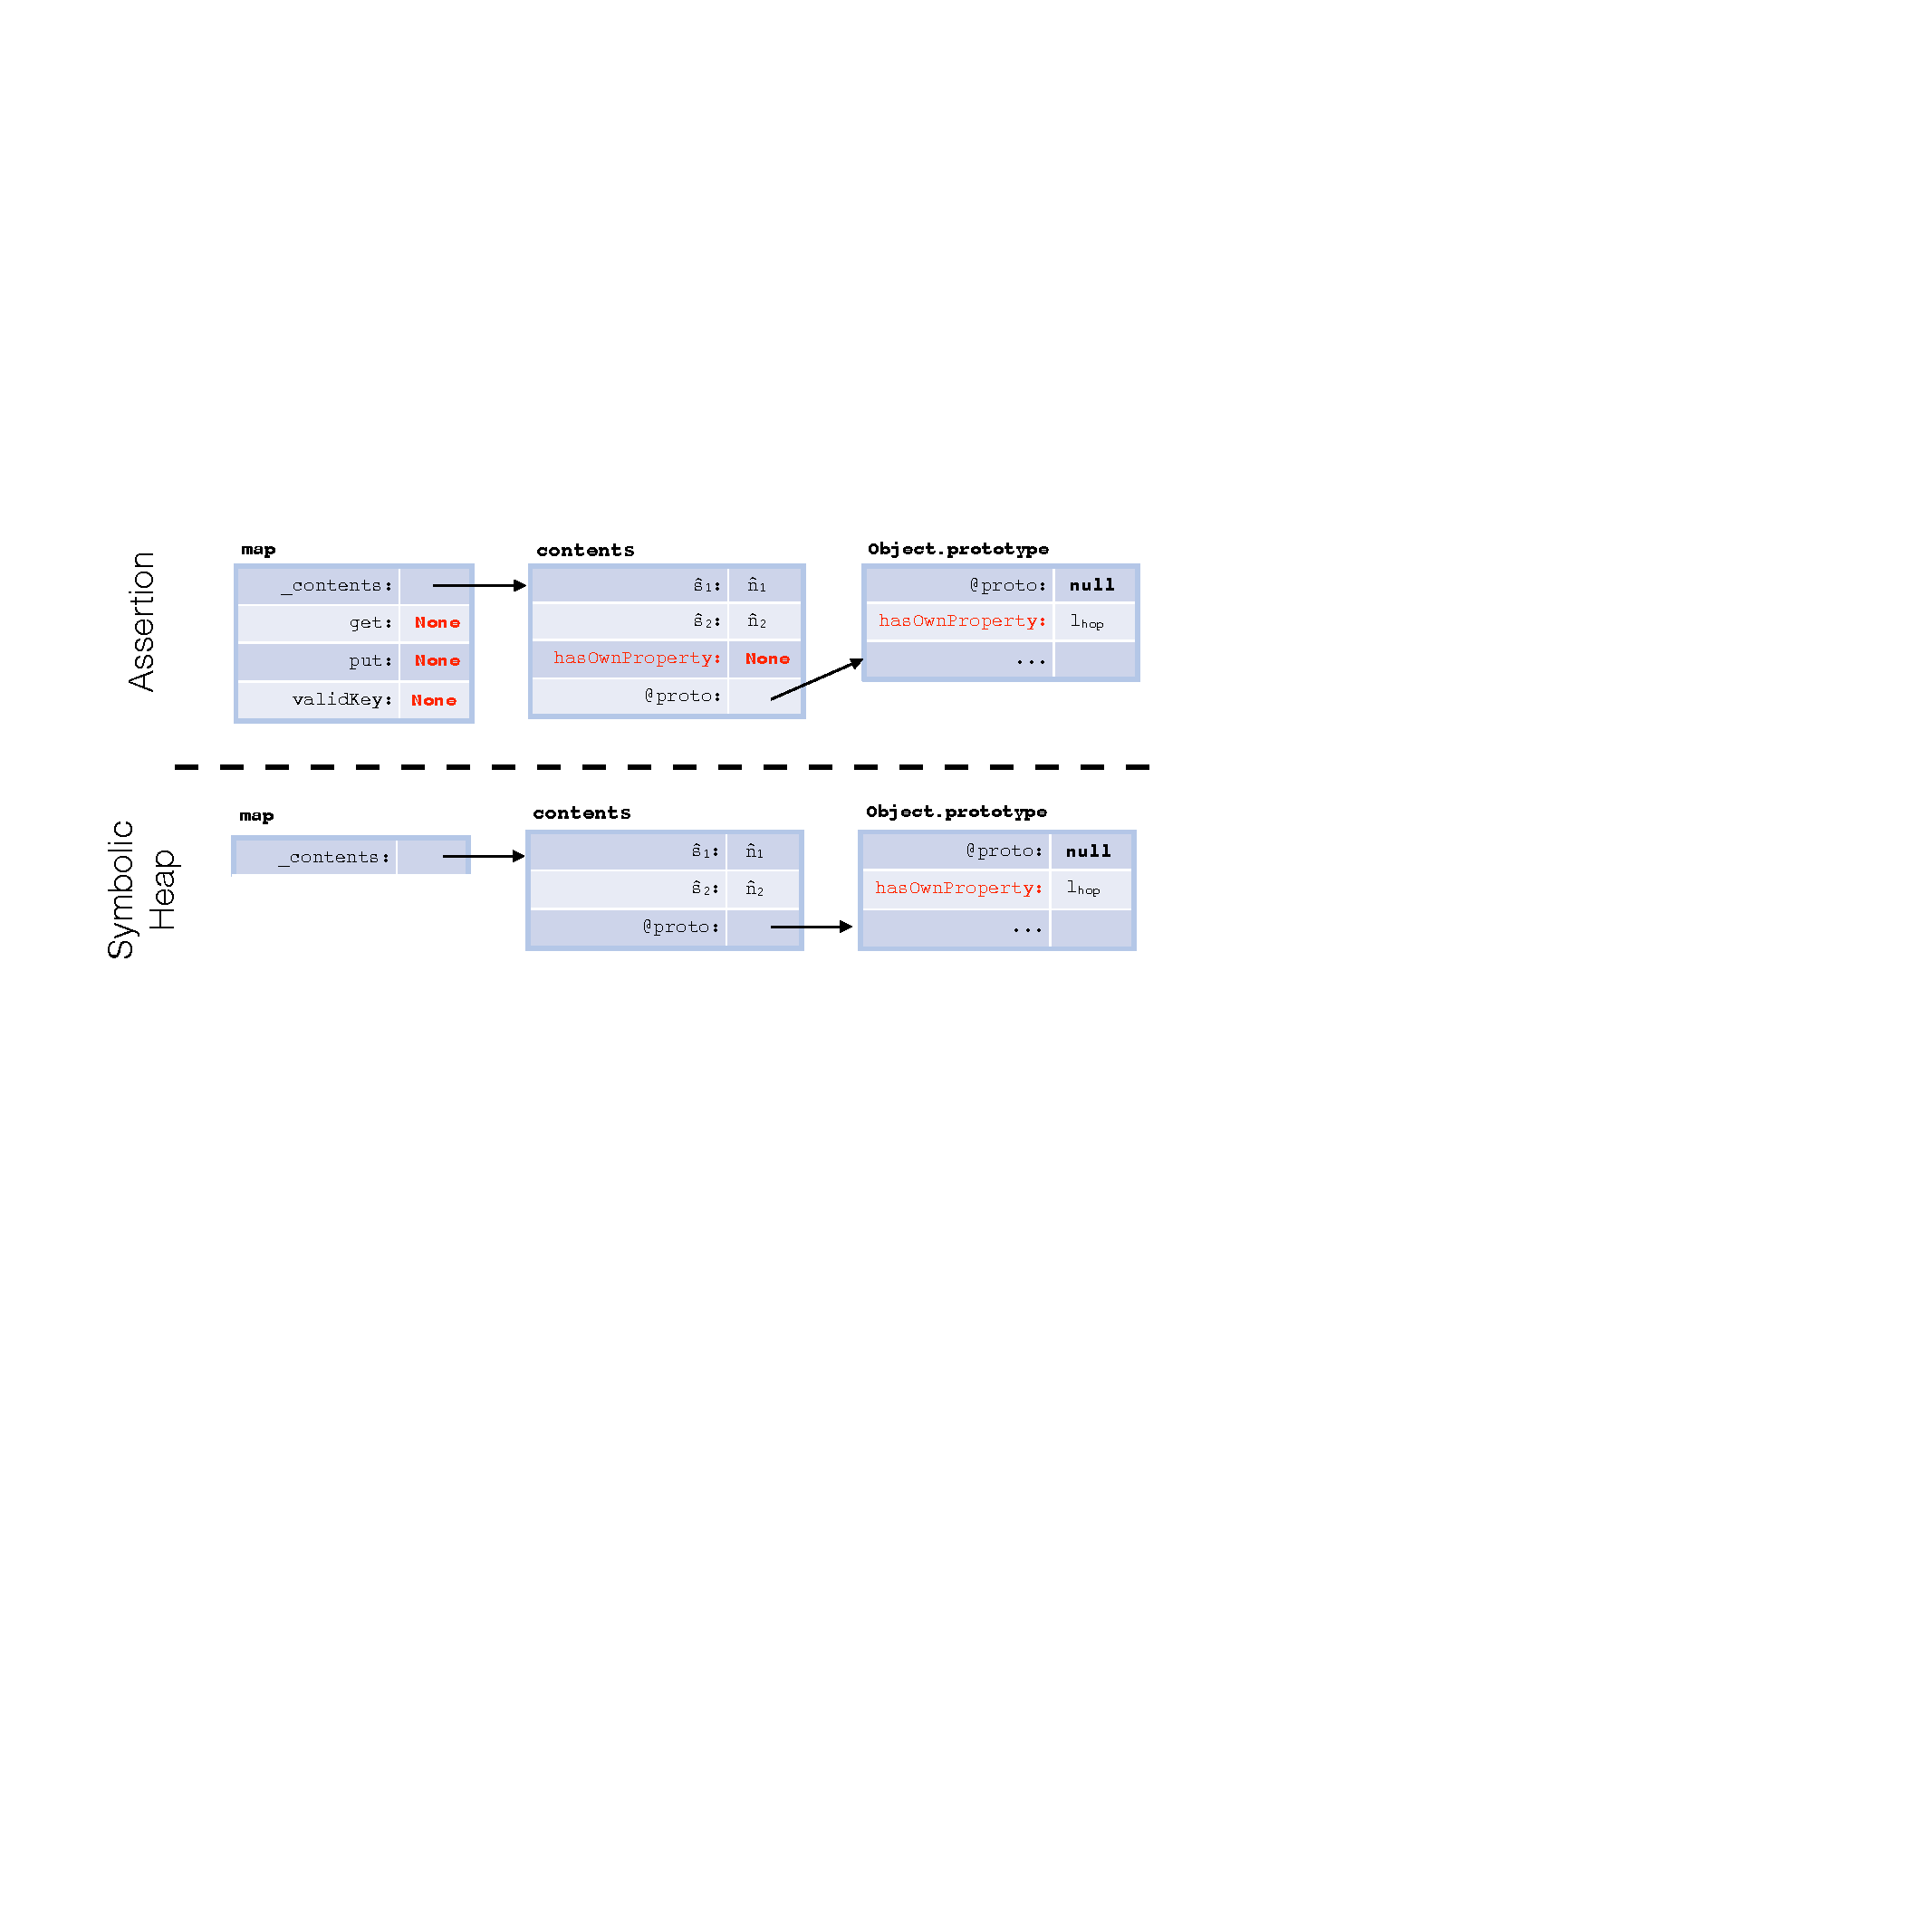
\includegraphics[width=0.9\textwidth]{figures/symbolicvsass.pdf}
{\small $$
\text{\emph{None-Constraints: }} (\hat{s}_1 \neq \texttt{"hasOwnProperty"} \, \wedge \, \hat{s}_2 \neq \texttt{"hasOwnProperty"})
$$}
\vspace{-25pt}
\caption{Assertion vs. Symbolic Heap}
\end{figure}



%\begin{algorithm}
%\caption{Synthesising a symbolic test for: $\lconf{P} \, \fid(\jvec{x}) \,  \lconf{Q}$}\label{infer:specs:algo}
%\begin{algorithmic}[1]
%\State $(\existentials, \sfs, \pfs) := \normalise(P)$ 
%\State $\sheap_0, \pfs_0, \theta := \concretise{(\existentials, \sfs, \pfs)}{[ \ ]}$
%\State $\subst' := \subst\mid_{\domain(\subst) \backslash \existentials}$
%\State Return: 
%%\ForAll{$XXX$}
%%\If{$XXX$}
%  %\State $\{ P \} \, \pid() \, \{ Q \} = \ispecs(\pid, \_)$
%%\Else
%  %\State $P,Q :=$
%%\EndIf
%%\State $ := InferSpec, \ispecs', \pid, P) $
%%\ForAll{$(Q_f,,\flag) \in $}
%%\If{$Q_f \sep Q_M \vdash Q \sep \true$}
%  %\State $\ispecs' := \ispecs' \cup \{(\pid, \flag) \mapsto {P \sep _f \sep Q_M}{\pid(\jvec{\xivar})}{Q_f \sep Q_M}\}$
%%\EndIf
%%\EndFor
%%\EndFor
%\end{algorithmic}
%\end{algorithm}


\subsection{Generating Symbolic Tests from JavaScript} 
\label{specs:example}

\myparagraph{Example}
In Figure~\ref{fig:map:example}, we define a \emph{map object predicate}, \jsinline|Map|, 
using the auxiliary predicate \jsinline|KVPairs|, which captures the resource of the key-value pairs in the map, 
and the \jsinline|validKey(k)| predicate, which holds if and only if the 
JavaScript function \jsinline|ValidKey(k)| returns \jsinline|true|\footnote{We treat the $\mathtt{ValidKey}$ predicate as a black box.}.
%
Intuitively, the \jsinline|Map(m, mp, kvs, keys)| predicate captures the resource 
of a map object \jsinline|m| with prototype \jsinline|mp|, keys \jsinline|keys| (a set of strings),
and key-value pairs \jsinline|kvs| (a set of string pairs\footnote{We model pairs as lists with two elements and, for clarity, use the pair notation.}). 
Observe that the definition of \jsinline|Map| does not include the resource of a map prototype, as
it is shared between all map objects, and therefore needs to be factored out.  
%
We write \jsinline|-u-| for set union and omit the brackets around singleton 
sets when the meaning is clear. % from the context. 

\begin{figure}[t!]
{\scriptsize
 \begin{verbatim}
Map (m, mp, kvs, keys) := JSObject(m, mp) * 
  DataProp(m, "_contents", c) * JSObject(c, Object.prototype) * KVPairs(c, kvs, keys) *
  (m, "get") -> None * (m, "put") ->  None * (m, "validKey") ->  None * 
  (c, "hasOwnProperty") ->  None *  emptyFields(c, keys -u- "hasOwnProperty")
  \end{verbatim}
  \vspace*{-0.3cm}
 \begin{verbatim}
KVPairs (o, kvs, keys) := 
  (kvs = { }) * (keys = { }),
  (kvs = (key, value) -u- kvs') * (keys = key -u- keys') * 
    ValidKey(key) * DataProp(o, key, value) * KVPairs(o, kvs', keys')
\end{verbatim}}
\caption{Map predicate \label{fig:map:example}}
\end{figure}

%In the following, we assume a \jsinline|MapProto| predicate specifying the resource of 
%a valid map prototype. In particular, the map prototype needs to define the methods 
%\jsinline|put|, \jsinline|get|, and \jsinline|validKey|. 


We are now in the position to specify the functions of the map library. In particular, below we show how to use 
the map object predicate to specify \jsinline|get(k)|.  
%
We consider the case in which the key whose value we  want to fetch is stored in the 
map.  The specification is given below. 
%
\begin{displaymath} 
{\footnotesize
\begin{array}{c}
\left\{ {\begin{array}{c}
 \text{\texttt{Map(this, mp, kvs -u- (k, v), ks) * ObjProtoF()}} \\ 
\end{array}} \right\} \\
%
\text{\bfseries \texttt{get(k)}} \\[0.2mm]
%
\left\{ {\begin{array}{c}
 \text{\texttt{Map(this, mp, kvs -u- (k, v), ks) * ObjProtoF() * (ret = v) }} \\
\end{array}} \right\}
\end{array}
} 
\end{displaymath}
%
The predicate \jsinline|ObjProtoF()| describes the resource captured by the \jsinline|Object.prototype| object. 
In particular, it is needed because \texttt{get} uses the \texttt{hasOwnProperty} function.



%%
%% OLD THINGS

%\begin{figure}[t!]
%\centering
%{\scriptsize
%\begin{mathpar} 
%\inferrule[\textsc{New Existential}]
%     { 
%         \svar \in \existentials 
%         \quad
%         \svar \not\in \domain(\subst)
%     }
%     {\unification{\sexpr, \pc}{\svar}{\subst}{\existentials} = \optionsome{\subst[\svar \mapsto \sexpr]}}
%\quad
%\inferrule[\textsc{Matched Existential}]
%     { 
%         \subst(\svar) = \sexpr' 
%         \quad 
%         \pc \vdash \sexpr = \sexpr' 
%     }
%     {\unification{\sexpr, \pc}{\svar}{\subst}{\existentials} = \optionsome{\subst}}
%\quad
%\inferrule[\textsc{Existential - None}]
%     { 
%         \subst(\svar) = \sexpr' 
%         \quad 
%         \pc \vdash \sexpr \neq \sexpr' 
%     }
%     {\unificationfail{\sexpr, \pc}{\svar}{\subst}{\existentials} = \optionnone}
%\\
%\inferrule[\textsc{Grounded Expression}]
%     { 
%         \fv(\subst(\sexpr')) \cap \existentials = \emptyset
%         \quad 
%          \pc \vdash  \sexpr = \subst(\sexpr') 
%     }
%     {\unification{\sexpr, \pc}{\sexpr'}{\subst}{\existentials} = \optionsome{\subst}}
%\qquad
%\inferrule[\textsc{Grounded Expression - Fail}]
%     { 
%         \fv(\subst(\sexpr')) \cap \existentials = \emptyset
%         \quad 
%          \pc  \vdash  \sexpr \neq \subst(\sexpr') 
%     }
%     {\unification{\sexpr, \pc}{\sexpr'}{\subst}{\existentials} = \optionnone}
%%
%\\
%\inferrule[\textsc{Cell Assertion}]
%	{  
%	   \big(\loc = \symbeval{\lexpr_l}{\sstore} \ \vee \loc = \subst(\symbeval{\lexpr_l}{\sstore}) \big)
%	   \quad 
%	     \symbeval{\lexpr_p}{\sstore} = \sexprp'
%	   \quad
%	   \symbeval{\lexpr_v}{\sstore} = \sexprv' 
%	   \quad
%	    \sheap = \sheap_f \dunion ((l, \sexprp) \mapsto \sexprv) 
%	   \\
%	   \unification{\sexprp, \pc}{\sexprp'}{\subst}{\existentials} = \optionsome{\subst'} 
%	   \quad
%	   \unification{\sexprv, \pc}{\sexprv'}{\subst'}{\existentials} = \optionsome{\subst''} 
%	}{ \unification{\sheap, \sstore, \pc}{(\lexpr_l,\lexpr_p)\pointsto \lexpr_v}{\subst}{\existentials} = \optionsome{(\subst'', \sheap_f)}} 
%\\
%\inferrule[\textsc{Cell Assertion - Fail}]
%	{  
%	   \big(\loc = \symbeval{\lexpr_l}{\sstore} \ \vee \loc = \subst(\symbeval{\lexpr_l}{\sstore}) \big)
%	   \quad
%	     \symbeval{\lexpr_p}{\sstore} = \sexprp'
%	   \quad
%	   \symbeval{\lexpr_v}{\sstore} = \sexprv' 
%	   \quad
%	     \sheap = \sheap' \dunion  \big((l, \sexprp_i) \mapsto \sexprv_i\big)\mid_{i = 0}^n   
%  	   \\
%	    (l, -) \not\in \domain(\sheap') 
%	    \quad 
%	   \forall_{0 \leq i \leq n} \, \unification{\sexprp, \pc}{\sexprp'}{\subst}{\existentials} = \optionnone 
%	   \ \vee \
%	   \unification{\sexprv, \pc}{\sexprv'}{\subst'}{\existentials} = \optionnone
%	}{ \unification{\sheap, \sstore, \pc}{(\lexpr_l,\lexpr_p)\pointsto \lexpr_v}{\subst}{\existentials} = \optionnone} 
%\\
%\inferrule[\textsc{EmptyFields Assertion}]
%	{  
%	   \big(\loc = \symbeval{\lexpr_l}{\sstore} \ \vee \loc = \subst(\symbeval{\lexpr_l}{\sstore}) \big)
%	   \quad 
%	     \symbeval{\lexpr_d}{\sstore} = \sexprv' 
%	   \\\\
%	     \sheap = \sheap' \, \uplus \, \big((l, \sexprp_i) \mapsto \sexprv_i\big)\mid_{i = 0}^n   
%              \quad
%             (l, -) \not\in \domain(\sheap')
%	    \quad 
%	    \pc \vdash \big( \{ \sexprp_i \mid_{i = 0}^n   \} \subseteq \sexprv' \big)
%	}{ \unification{\sheap, \sstore, \pc}{\emptyfields{\lexpr_l}{\lexpr_d}}{\subst}{\existentials} = \optionsome{(\subst, \sheap)}} 
%\\
%\inferrule[\textsc{EmptyFields Assertion - Failing}]
%	{  
%	   \big(\loc = \symbeval{\lexpr_l}{\sstore} \ \vee \loc = \subst(\symbeval{\lexpr_l}{\sstore}) \big)
%	   \quad 
%	     \symbeval{\lexpr_d}{\sstore} = \sexprv' 
%	   \\\\
%	     \sheap = \sheap' \, \uplus \, \big((l, \sexprp_i) \mapsto \sexprv_i\big)\mid_{i = 0}^n   
%              \quad
%             (l, -) \not\in \domain(\sheap')
%	    \quad 
%	    \pc \vdash \big( \{ \sexprp_i \mid_{i = 0}^n   \} \not\subseteq \sexprv' \big)
%	}{ \unification{\sheap, \sstore, \pc}{\emptyfields{\lexpr_l}{\lexpr_d}}{\subst}{\existentials} = \optionnone} 
%\end{mathpar}
%\hrule
%\caption{Unification of spatial assertions:
% {\scriptsize$\unification{\sheap, \sstore, \pc}{\cell}{\subst}{\existentials} = (\subst', \sheap_f)$}\label{fig:unification}}}
%\end{figure}


%{\small 
%\begin{align}
%\sepmodels{P} = \left\{ (\iheap, \store) \mid \exists \senv \, . \,  \iheap, \store, \senv \satisfies P  \right\} 
%\\ 
%\smodels{\isheap, \sstore}{\pc} = \left\{ (\iheap, \store) \mid \exists \senv \, . \,  \senv \vdash \pc \ \wedge \
%    \iheap = \symbeval{\isheap}{\senv} \ \wedge \ \store = \symbeval{\sstore}{\senv}  \right\} 
%\end{align}} 



%
%\begin{figure}
%{\scriptsize
%\centering
%\begin{mathpar} 
%\inferrule[\textsc{Spatial Assertion}]
%	{  
%	   \unification{\sheap, \sstore, \pc}{(\lexpr_l,\lexpr_p)\pointsto \lexpr_v}{\subst} = \uyes{\sheap_f}
%	}{\cellunification{\sheap, \cell \lstcons \cells}{\sheap_q, \cells}{\sstore, \pc, \subst}} 
%\\
%\inferrule[\textsc{Successful Unification}]
%	{  
%	   
%	   \cellunificationiter{\sheap, \cells}{\hemp, []}{\sstore, \pc, \subst}
%	   \qquad 
%	   \pc \vdash \subst(\pfs')
%%	   \cells =  \cell \lstcons \cells'
%%	   \and
%%            \unification{\sheap, \sstore, \pc}{\cell}{\subst} = \uyes{\sheap_f}
%%            \\\\
%%            \unificationfull{\sheap_f, \sstore, \pc}{\cells', \pfs'}{\subst}
%	}{\unificationfull{\sheap, \sstore, \pc}{\cells, \pfs'}{\subst}} 
%\and 
%\inferrule[\textsc{Spatial Assertion}]
%	{  
%	   \cells = \cell \lstcons \cells'
%	   \and
%            \unification{\sheap, \sstore, \pc}{\cell}{\subst} = \uyes{\sheap_f}
%            \\\\
%            \unificationfullfail{\sheap_f, \sstore, \pc}{\cells', \pfs'}{\subst}{\pc'}
%	}{\unificationfullfail{\sheap, \sstore, \pc}{\cells, \pfs'}{\subst}{\pc'}} 
%\\
%\inferrule[\textsc{Pure Assertions}]
%	{  
%	   \pc \vdash \subst(\pfs')
%	}{\unificationfull{\hemp, \sstore, \pc}{\emptyset, \pfs'}{\subst}} 
%%
%\and
%%
%\qquad
%\inferrule[\textsc{Pure Assertions -  Fail}]
%	{  
%	      \pc \not\vdash \subst(\pfs')
%	}{\unificationfullfail{\sheap, \sstore, \pc}{\emptyset, \pfs'}{\subst}{\subst(\pfs')}} 
%\\
%%
%\inferrule[\textsc{Cell Assertion - Fail}]
%	{  
%	   \sfs = \cells \lstcons \cells
%	   \and
%            \unification{\sheap, \sstore, \pc}{\cell}{\subst} = \uno{\pc'}
%	}{\unificationfullfail{\sheap, \sstore, \pc}{\sfs, \pfs'}{\subst}{\pc'}} 
%%
%\and
%\inferrule[\textsc{Extra Resource -  Fail}]
%	{  
%	    \sheap \neq \hemp
%	}{\unificationfullfail{\sheap, \sstore, \pc}{\emptyset, \pfs'}{\subst}{\jtrue}} 
%%
%\end{mathpar}}
%\hrule



\newpage
\section{Evaluation}
%!TEX root = ../main.tex

We discuss the trustworthiness of \cosette and demonstrate that~our implementation, despite being  a proof-of-concept, has already proven useful for the debugging of real-world JavaScript code.
We elaborate on the results presented below in more detail in the Appendix. 

\myparagraph{Trustworthiness: JavaScript Semantics}
To ensure that Cosette follows the semantics of JavaScript without any simplifications, we tested \JSComp and our instrumented \jsil interpreter implemented in Rosette using Test262, the JavaScript official test suite~\cite{test262}. 
Out of the 10469 tests for ES5 Strict, we have identified 8330 tests appropriate for our coverage, of which we pass 100\%.

\myparagraph{Trustworthiness: Symbolic Interpreter} To make certain that the symbolic \jsil interpreter obtained by the Rosette lifting of the implemented instrumented interpreter is consistent with the symbolic semantics of \S\ref{subsec:symb:semantics}, we systematically constructed and successfully ran symbolic unit tests for each \jsil command, assuming the premises and asserting the conclusion of the appropriate rule of the symbolic semantics.

%With \cosette, we can write symbolic tests, in which some of the concrete values of the program are replaced with symbolic values.
%Symbolic tests improve on concrete tests for two main reasons.
%First, they are by construction more comprehensive than concrete tests, because symbolic tests can account for the whole range of values that a variable can take, instead of focusing on a few specific examples.
%Second, when \cosette finds a failing assertion inside a symbolic test, it can concretize the symbolic values into a counter-model that the developer can actually run in node, making debugging much easier compared to (the other things that we mention before).

\myparagraph{Whole-program Symbolic Testing: JS-Specific Features}
We created a number of symbolic tests to demonstrate that Cosette can reason about essential JavaScript features, such as prototype inheritance, function closures, arrays, strings, as well as the substantially more challenging for-in statement and dynamic dispatch. 

\myparagraph{Whole-program Symbolic Testing: Real-World Libraries}
We used \cosette to analyse the code of two JavaScript data structure libraries: Buckets.js~\cite{buckets}, and queue-pri~\cite{priq}.
We chose these libraries because reasoning about data structure code requires a precise description of the control flow features of JavaScript, because they come equipped with unit test suites, and because they do not have external dependencies (\cosette is a whole-program analysis); Buckets.js has over 65k downloads on npm.

For these two libraries, we wrote symbolic tests with the aim of obtaining a line coverage of 100\%, in order to compare them with the concrete unit tests that ship with the libraries.
In both cases, we were able to reduce the length of the tests by up to an average factor of 3, while increasing line coverage from around 90\% to a full 100\%.
We also discovered one bug in the Buckets.js library, as well as one in the queue-pri library.


The results are presented in table~\ref{cosette:res}.
For each file in the library, we report the number of JS executable lines in the code itself and including dependencies (slash-separated), the corresponding numbers of JSIL lines, the number of symbolic and concrete test cases, the number of JS lines in the symbolic and concrete tests, the coverage measured as percentage of lines and the average \cosette run time for the symbolic tests.
The files in Buckets.js are separated by a line from the unique file in queue-pri.

For the testing, we used a machine with an Intel Core i7-4980HQ CPU 2.80 GHz and DDR3 RAM 16GB. We measured the execution time of each symbolic test and averaged the times across tests for each library file. The times that we obtained reflect the fact that Rosette code is interpreted, rather than being run natively. We aim at implementing our own symbolic execution tool from scratch in the future, which, given our experience with JaVerT, should reduce execution times by at least an order of magnitude.

\begin{table}[!t]
{
\small
%\begin{center}
\setlength\tabcolsep{4pt}
\begin{tabular*}{\linewidth}{l@{\;\;}rrrrrr}
\toprule
% Name || JS Loc/loc* || JSIL Loc/loc* || #tests || symb/conc loc || symb/conc cov || time
Name & \makecell{JS lines} & \makecell{JSIL lines} & \# Tests & \makecell{Test lines} & \makecell{Line\\Cov.~(\%)} & \makecell{Avg.\\time} \\
\midrule
\texttt{arrays} & 44/71 & 1251/1942 & 9/24 & 166/329 & 100/100 & 20s \\
\texttt{bag} & 69/237 & 2041/7194 & 7/18 & 78/265 & 100/76.8 & 74s \\
\texttt{bstree} & 143/326 & 3819/8052 & 11/31 & 216/759 & 100/98.6 & 5m27s \\
\texttt{dict} & 57/84 & 1683/2374 & 7/14 & 116/170 & 100/80.7 & 15s \\
\texttt{heap} & 57/128 & 2059/4001 & 4/15 & 92/626 & 100/96.5 & 5m29s \\
\texttt{llist} & 126/153 & 2447/3138 & 9/21 & 149/370 & 100/94.4 & 24s \\
\texttt{multidict} & 56/184 & 1871/5496 & 6/16 & 118/189 & 100/74.1 & 1m15s \\
\texttt{pqueue} & 26/154 & 1066/5067 & 5/12 & 70/283 & 100/96.2 & 5m49s \\
\texttt{queue} & 30/183 & 1095/4233 & 6/9 & 111/146 & 100/96.7 & 20s \\
\texttt{set} & 40/124 & 1528/3902 & 6/12 & 86/271 & 100/70.0 & 1m01s \\
\texttt{stack} & 23/176 & 941/4079 & 4/7 & 91/104 & 100/87.0 & 26s \\
\midrule 
\texttt{queue-pri} & 19/164 & 872/5086 & 2/9 & 26/80 & 100/100 & xy.z \\
\bottomrule
%\end{center}
\end{tabular*}
}
\caption{Tests for the Buckets.js and queue-pri libraries}
\vspace*{-0.95cm}
\label{cosette:res}
\end{table}

%\pmax{Say something about how bugs work - sometimes coverage, sometimes semantics.}

\smallskip
\noindent \emph{Bug: MultiDictionary in Buckets.js.}
We have discovered a bug in the implementation of the Buckets.js multi-dictionary library.
A multi-dictionary is a key-value map in which a single key holds an array of distinct values. 
Our symbolic tests for the \jsinline|remove(key, value)| function, which removes a given key-value pair from the multi-dictionary, have revealed that the library wrongly treats the case in which we try to remove a key-value pair for a key with no associated values.
Concretely, a runtime error is thrown instead of \jsinline|remove| returning \jsinline|false|. 
This bug was not detected by the concrete unit tests associated with the library due to their incomplete coverage;
we have fixed it and submitted an appropriate pull request.




\smallskip
\noindent \emph{Bug: queue-pri.} This library implements a priority queue that stores data with an optional priority value.
The priority can either be a number (the lower the value, the higher the priority) or the default \jsinline{null} value if no priority is provided, in which case the associated element is put at the end of the queue. Our symbolic tests of the \jsinline{enqueue(data, pri)} method of the library have shown that that elements enqueued with priority \jsinline{0} were wrongly being always enqueued at the end of the queue. We traced the bug to the way in which priority was calculated inside \jsinline{enqueue}: \jsinline{priority = pri || null}, which evaluates to \jsinline|null| if the priority is not supplied, but also, due to the semantics of JavaScript, if it is equal to 0. This bug was not caught by the unit tests of the library because the developer had not considered inserting nodes with priority 0. This shows that \cosette is a useful tool for symbolic testing, because it fully follows the semantics of JavaScript and will expose corner cases that a developer may not be aware of.

\myparagraph{Specification-directed Bug-finding} 

\pmax{JaVerT examples - testing the unfolding, introducing bugs}

\newpage
\section{Related Work} 

The existing literature covers a wide range of analysis techniques for JavaScript programs, including: 
type systems~\cite{thiemann:esop:2005,anderson:ecoop:2005,jensen:sas:2009,typescript:toot:2014,feldthaus:oopsla:2014,bierman:ecoop:2014,rastogi:popl:2015},
control flow analysis~\cite{feldthaus2013efficient}, pointer analysis~\cite{jang2009points,sridharan:ecoop:12} and abstract
interpretation~\cite{kashyap:fse:14,jensen:sas:2009,andreasen:oopsla:2014,park:ecoop:15}, among others. 
Here, we focus on the existing work on logic-based analysis and symbolic execution for JavaScript. 

\myparagraph{Symbolic Execution} Ooga. Booga. Boo.




\myparagraph{Logic-based Analysis} 
%
\cite{gardner:popl:2012} have developed a separation logic for a small fragment of ECMAScript 3, to reason about the variable store emulated in the JavaScript heap.
%
\cite{rosu-serbanuta-2010-jlap} have developed $\mathbb{K}$, a term-rewriting framework  for  formalising the operational
semantics of programming languages.
 In particular, they have developed KJS~\cite{Park:2015} which provides a $\mathbb{K}$-interpretation of the core language and part of the built-in libraries of the ES5 standard. KJS has been tested against the official ECMAScript Test262 test suite and passed all 2782 tests for the core language; the testing results for the built-in libraries are not reported. 
\cite{stefanescu-park-yuwen-li-rosu-2016-oopsla} introduce a language-independent verification infrastructure 
that can be instantiated with a $\mathbb{K}$-interpretation of a  language to automatically generate a symbolic verification tool for that language based on the $\mathbb{K}$ reachability logic. They apply this infrastructure to KJS to generate a verification tool for JavaScript, which they use to verify functional correctness properties of operations for manipulating data structures such as binary search trees, AVL trees, and lists.


\section{Conclusions}\label{conclusions}

\pmaxinline{Can we be more general, and say something like 'logic-based specifications'? It's all about translating to FOL, or even some version of PL. Also, we need to say at some point why we care about specifications written in separation logic.}

\newpage
\bibliography{ecoop18}

\newpage
\appendix

%!TEX root = ../main.tex

\newtheorem{lemmax}{}
\newtheorem{temax}{}

\section{\jsil Syntax and Semantics}


\begin{figure}[ht!]
{\scriptsize
\begin{mathpar} 
%
\inferrule[\textsc{Skip}]{}
	{ \semtrans{\heap, \store, \jsilskip}{\heap, \store}} 
 \qquad
 %
\inferrule[\textsc{Assignment}]
  {
      \symbeval{\jsilexpr}{\store} =  \val
      \quad
      \store' = \store[\jvar \mapsto \val]
  }{\semtrans{\heap, \store, \jvar := \jsilexpr}{\heap, \store'}} 
%
\qquad 
%
\inferrule[\textsc{Object Creation}]
  { 
    \heap = \heap \dunion \hcell{\loc}{\protop}{\jsnull}
    \quad (\loc,-) \notin \domain (\heap)
  }{\semtrans{\heap, \store, \jvar := \jsilnew()}{\heap, \store[\jvar \mapsto \loc]}}
\\
%
\inferrule[\textsc{Property Access}]
  { 
 	\symbeval{\jsilexpr_1}{\store} =  \loc
  	\quad 
        \symbeval{\jsilexpr_2}{\store} =  \jstring
        \quad
        \heap = - \dunion \hcell{\loc}{\jstring}{\val}
  }{ \semtrans{\heap, \store, \jvar := [\jsilexpr_1, \jsilexpr_2]}{\heap,  \store[\jvar \mapsto \val]}}
 \and 
 \inferrule[\textsc{Property Deletion}]
  { 
        \symbeval{\jsilexpr_1}{\store} =  \loc
  	\quad 
        \symbeval{\jsilexpr_2}{\store} =  \jstring
        \quad
        \heap = \heap' \dunion \hcell{\loc}{\jstring}{-}
  }{\semtrans{\heap, \store, \jsildelete(\jsilexpr_1, \jsilexpr_2)}{\heap', \store}}
 %
\\
%
\inferrule[\textsc{Property Assignment - Found}]
  {     \symbeval{\jsilexpr_1}{\store} =  \loc
  	\quad 
        \symbeval{\jsilexpr_2}{\store} =  \jstring
        \quad
        \symbeval{\jsilexpr_3}{\store} =  \val
       \\\\
        \heap = \heap' \dunion  \hcell{\loc}{\jstring}{-}
  }{\semtrans{\heap, \store, [\jsilexpr_1, \jsilexpr_2] := \jsilexpr_3}{\heap' \dunion  \hcell{\loc}{\jstring}{\val}, \store}} 
 \and 
 \inferrule[\textsc{Property Assignment - Not Found}]
  {     \symbeval{\jsilexpr_1}{\store} =  \loc
  	\quad 
        \symbeval{\jsilexpr_2}{\store} =  \jstring
        \quad
        \symbeval{\jsilexpr_3}{\store} =  \val
       \\\\
        \heap = \heap' 
        \quad 
        (\loc, \jstring) \not\in \domain(\heap)
  }{\semtrans{\heap, \store, [\jsilexpr_1, \jsilexpr_2] := \jsilexpr_3}{\heap \dunion  \hcell{\loc}{\jstring}{\val}, \store}} 
\\
%
\inferrule[\textsc{Member Check - True}]
  { 
      \symbeval{\jsilexpr_1}{\store} =  \loc
  	\quad 
        \symbeval{\jsilexpr_2}{\store} =  \jstring
       \quad 
   	(\loc, \jstring) \in \domain(\heap) 
  }{\semtrans{\heap, \store,\jvar := \hasfield(\jsilexpr_1, \jsilexpr_2)}{\heap, \store[\jvar \mapsto \jtrue]}}
  \and 
 \inferrule[\textsc{Member Check - False}]
  { 
      \symbeval{\jsilexpr_1}{\store} =  \loc
  	\quad 
        \symbeval{\jsilexpr_2}{\store} =  \jstring
       \quad 
   	(\loc, \jstring) \not\in \domain(\heap) 
  }{\semtrans{\heap, \store,\jvar := \hasfield(\jsilexpr_1, \jsilexpr_2)}{\heap, \store[\jvar \mapsto \jfalse]}}
%
\\
%
\inferrule[\textsc{Assert - True}]
  { 
      \symbeval{\jsilexpr}{\store} =  \jtrue
  }{\semtrans{\heap, \store, \assert(\jsilexpr)}{\heap, \store}} 
\and
\inferrule[\textsc{Assert - False}]
  { 
      \symbeval{\jsilexpr}{\store} \neq \jtrue
  }{\semtranserr{\heap, \store, \assert(\jsilexpr)}} 
\end{mathpar}}
\caption{Symbolic Execution for Basic Commands: {\scriptsize$\semtrans{\heap, \store, \bcmd}{\heap', \store'}$}\label{fig:sem:basic:commands}}
\end{figure}




\begin{figure}[ht!]
{\scriptsize
\begin{mathpar} 
\inferrule[\textsc{Basic Command}]
   { 
     \prog_{\pid}(i) = \bcmd 
     \quad
     \semtrans{\heap, \store, \bcmd}{\heap', \store'} 
   }{\semtrans{\heap, \store, \ctx[i]}{\heap', \store', \ctx[i+1]}}
%
   \qquad
  %
  \inferrule[\textsc{Basic Command - Fail}]
   { 
     \prog_{\pid}(i) = \bcmd 
     \quad
     \semtranserr{\heap, \store, \bcmd} 
   }{\semtranserr{\heap, \store, \ctx[i]}}
 %
   \qquad
  %
  \inferrule[\textsc{Goto}]
   { \prog_{\pid}(i) = \goto \, j \quad}
   {\semtrans{\heap, \store, \ctx[i]}{\heap, \store, \ctx[j]}}
  \\ 
  \inferrule[\textsc{Cond. Goto - True}]
   { \prog_{\pid}(i) =  \ifgoto{\jsilexpr}{j}{k} \quad
     \symbeval{\jsilexpr}{\store} =  \jtrue
   }
   {\semtrans{\heap, \store, \ctx[i]}{\heap, \store, \ctx[j]}}
  \and 
    \inferrule[\textsc{Cond. Goto - False}]
   { \prog_{\pid}(i) =  \ifgoto{\jsilexpr}{j}{k} \quad
     \symbeval{\jsilexpr}{\store} =  \jfalse
   }
   {\semtrans{\heap, \store, \ctx[i]}{\heap, \store, \ctx[k]}}
   \\
    \inferrule[\textsc{Procedure Call}]
   { 
    \prog_{\pid}(i) =   \jsilcall{\jvar}{\jsilexpr}{\jsilexpr_i \mid_{i = 0}^{n}}{j}
     \quad
    \symbeval{\jsilexpr}{\sstore} =  \pid' 
        \quad
     \args(\pid') = \jsillist{\jvar_1, ..., \jvar_{m}} 
      \quad
      \val_i = \symbeval{\jsilexpr_i}{\sstore} \mid_{i = 0}^{n} 
     \ 
      \val_i = \jsundefined \mid_{i = n+1}^{m}  
   }
   {\semtrans{\heap, \store, \ctx[i]}{\heap, [ \jvar_i \mapsto \val_i \mid_{i = 0}^{m}] , ((\pid', \store, \jvar, i+1, j)::\ctx)[0]}}
    \\ 
  \inferrule[\textsc{Normal Return}]
   {
       \ctx = (-, \store', \jvar, i, -) :: \ctx' 
       \quad 
       \store(\procretvar) = \val
   }  
   {\semtrans{\heap, \store, \ctx[\procretlab]}{\heap, \store'[\jvar \mapsto \val], \ctx'[i]}}
   \and 
     \inferrule[\textsc{Error Return}]
   {
       \ctx = (-, \store', \jvar, -, j) :: \sctx' 
       \quad 
       \sstore(\procerrvar) = \val
   }
   {\semtrans{\heap, \store, \ctx[\procerrlab]}{\sheap, \store'[\jvar \mapsto \val], \ctx'[j]}}
 \end{mathpar}}
\caption{Symbolic Execution for Control Flow Commands: {\scriptsize$\semtrans{\heap, \store, \ctx[i]}{\heap', \store', \ctx'[j]}$}} 
\end{figure}


\begin{figure}[ht!]
{\scriptsize
\begin{mathpar} 
\inferrule[\textsc{Basic Command}]
   { 
     \ccmd[\prog][\ctx]{i} = \bcmd 
     \quad
     \semtrans{\heap, \store, \bcmd}{\heap', \store'} 
   }{\semtrans[\prog]{\heap, \store, i}{\heap', \store', i+1}[C]}
%
   \qquad
  %
  \inferrule[\textsc{Basic Command - Fail}]
   { 
     \ccmd[\prog][\ctx]{i} = \bcmd 
     \quad
     \semtranserr{\heap, \store, \bcmd} 
   }{\semtranserr[\prog]{\heap, \store, i}[C]}
 %
   \qquad
  %
  \inferrule[\textsc{Goto}]
   { \ccmd[\prog][\ctx]{i} = \goto \, j \quad}
   {\semtrans[\prog]{\heap, \store, i}{\heap, \store, j}[C]}
  \\ 
  \inferrule[\textsc{Cond. Goto - True}]
   { \ccmd[\prog][\ctx]{i} =  \ifgoto{\jsilexpr}{j}{k} \quad
     \symbeval{\jsilexpr}{\store} =  \jtrue
   }
   {\semtrans[\prog]{\heap, \store, i}{\heap, \store, j}[C]}
  \and 
    \inferrule[\textsc{Cond. Goto - False}]
   { \ccmd[\prog][\ctx]{i} =  \ifgoto{\jsilexpr}{j}{k} \quad
     \symbeval{\jsilexpr}{\store} =  \jfalse
   }
   {\semtrans[\prog]{\heap, \store, i}{\heap, \store, k}[C]}
   \\
    \inferrule[\textsc{Procedure Call}]
   { 
    \ccmd[\prog][\ctx]{i} =   \jsilcall{\jvar}{\jsilexpr}{\jsilexpr_i \mid_{i = 0}^{n}}{j}
     \quad
    \symbeval{\jsilexpr}{\sstore} =  \pid' 
        \quad
     \args(\pid') = \jsillist{\jvar_1, ..., \jvar_{m}} 
      \quad
      \val_i = \symbeval{\jsilexpr_i}{\sstore} \mid_{i = 0}^{n} 
     \ 
      \val_i = \jsundefined \mid_{i = n+1}^{m}  
   }
   {\semtrans[\prog]{\heap, \store, i}{\heap, [ \jvar_i \mapsto \val_i \mid_{i = 0}^{m}] , 0}[C][(\pid', \store, \jvar, i+1, j) :: \ctx]}
    \\ 
  \inferrule[\textsc{Normal Return}]
   {
       \ctx = (-, \store', \jvar, i, -) :: \ctx' 
       \quad 
       \store(\procretvar) = \val
   }  
   {\semtrans[\prog]{\heap, \store, \procretlab}{\heap, \store'[\jvar \mapsto \val], i}[C][C']}
   \and 
     \inferrule[\textsc{Error Return}]
   {
       \ctx = (-, \store', \jvar, -, j) :: \ctx' 
       \quad 
       \store(\procerrvar) = \val
   }
   {\semtrans[\prog]{\heap, \store, \procerrlab}{\heap, \store'[\jvar \mapsto \val], j}[C][C']}
 \end{mathpar}}
 \pmax{What happens when we exit from main, how do we stop? Basically, cmd, returns nothing and we can't reduce?}
 \vspace*{-0.4cm}
\caption{Symbolic Execution for Control Flow Commands: $\semtrans[\prog]{\heap, \store, i}{\heap', \store', j}[C][C']$}
\end{figure}

\begin{figure}[ht!]
{\scriptsize
\begin{mathpar} 
\inferrule[\textsc{Basic Command}]
   { 
     \ccmd{i} = \bcmd 
     \quad
     \semtrans{\heap, \store, \bcmd}{\heap', \store'} 
   }{\semtrans{\heap, \store, i}{\heap', \store', i+1}}
%
   \qquad
  %
  \inferrule[\textsc{Basic Command - Fail}]
   { 
     \ccmd{i} = \bcmd 
     \quad
     \semtranserr{\heap, \store, \bcmd} 
   }{\semtranserr{\heap, \store, i}}
 %
   \qquad
  %
  \inferrule[\textsc{Goto}]
   { \ccmd{i} = \goto \, j \quad}
   {\semtrans{\heap, \store, i}{\heap, \store, j}}
  \\ 
  \inferrule[\textsc{Cond. Goto - True}]
   { \ccmd{i} =  \ifgoto{\jsilexpr}{j}{k} \quad
     \symbeval{\jsilexpr}{\store} =  \jtrue
   }
   {\semtrans{\heap, \store, i}{\heap, \store, j}}
  \and 
    \inferrule[\textsc{Cond. Goto - False}]
   { \ccmd{i} =  \ifgoto{\jsilexpr}{j}{k} \quad
     \symbeval{\jsilexpr}{\store} =  \jfalse
   }
   {\semtrans{\heap, \store, i}{\heap, \store, k}}
   \\
    \inferrule[\textsc{Procedure Call}]
   { 
    \ccmd{i} = \jsilcall{\jvar}{\jsilexpr}{\jsilexpr_i \mid_{i = 0}^{n}}{j}
     \quad
    \symbeval{\jsilexpr}{\sstore} =  \pid' 
        \quad
     \args(\pid') = \jsillist{\jvar_1, ..., \jvar_{m}} 
      \quad
      \val_i = \symbeval{\jsilexpr_i}{\sstore} \mid_{i = 0}^{n} 
     \ 
      \val_i = \jsundefined \mid_{i = n+1}^{m}  
   }
   {\semtrans{\heap, \store, i}{\heap, [ \jvar_i \mapsto \val_i \mid_{i = 0}^{m}] , 0}[C][(\pid', \store, \jvar, i+1, j) :: \ctx]}
    \\ 
  \inferrule[\textsc{Normal Return}]
   {
       \ctx = (-, \store', \jvar, i, -) :: \ctx' 
       \quad 
       \store(\procretvar) = \val
   }  
   {\semtrans{\heap, \store, \procretlab}{\heap, \store'[\jvar \mapsto \val], i}[C][C']}
   \and 
     \inferrule[\textsc{Error Return}]
   {
       \ctx = (-, \store', \jvar, -, j) :: \ctx' 
       \quad 
       \store(\procerrvar) = \val
   }
   {\semtrans{\heap, \store, \procerrlab}{\heap, \store'[\jvar \mapsto \val], j}[C][C']}
 \end{mathpar}}
 \vspace*{-0.4cm}
\caption{Symbolic Execution for Control Flow Commands: $\semtrans[\prog]{\heap, \store, i}{\heap', \store', j}[C][C']$}
\end{figure}

\section{Proofs - Section~\ref{sec:jsil:symb:exec}}

\begin{lemma}[Soundess of symbolic execution for \jsil basic commands]\label{soundness:basic:commands}
$$
\begin{array}{l}
\symbtrans{\sheap, \sstore, \bcmd, \pc}{\sheap', \sstore', \pc'}
   \ \wedge \ 
      (\heap, \store) \in \smodels{\sheap, \sstore}{\pc'} \\ \quad \quad
      	 \ \implies \ \exists (\heap', \store') \, . \, 
	 	 \semtrans{\heap, \store, \bcmd}{\heap', \store'}
		\, \wedge \, 
		(\heap', \store') \in \smodels{\sheap', \sstore'}{\pc'}  
\end{array}
$$
\end{lemma}
\begin{proof}
We proceed by case analysis on $\symbtrans{\sheap, \sstore, \bcmd, \pc}{\sheap', \sstore', \pc'}$. 
\vspace{5pt}

\noindent\prooflab{Skip} 
We conclude that $\bcmd = \jsilskip$, and 
that $\sheap' = \sheap$, $\sstore' = \sstore$, and $\pc' = \pc$. 
By picking $\heap' = \heap$, $\store' = \store$, the result follows. 
\vspace{6pt}

\noindent\prooflab{Assignment} 
We conclude that $\bcmd = \jvar := \jsilexpr$, for some variable $\jvar$ and expression $\jsilexpr$, 
and that $\sheap' = \sheap$, $\sstore' = \sstore[\jvar \mapsto \symbeval{\jsilexpr}{\store}]$, and $\pc' = \pc$. 
From $(\heap, \store) \in \smodels{\sheap, \sstore}{\pc'}$, we conclude that there is a symbolic environment 
$\senv$ such that $\heap = \semexpr{\sheap}{\senv}$ and $\store = \semexpr{\sstore}{\senv}$. 
Noting that: 
$$
 \semtrans{\heap, \store, \jvar := \jsilexpr}{\heap, \store[\jvar \mapsto \symbeval{\jsilexpr}{\store}]}
% \qquad 
 %\semexpr{\sstore[\jvar \mapsto \symbeval{\jsilexpr}{\store}]}{\senv} = \semexpr{\sstore}{\senv}[\jvar \mapsto \symbeval{\jsilexpr}{\store, \senv}]
$$
we pick $\heap' = \heap$ and $\store' =  \store[\jvar \mapsto \symbeval{\jsilexpr}{\store}]$. We 
now have to prove that $(\heap', \store') \in \smodels{\sheap', \sstore'}{\pc}$.
Observing that: 
$$
\heap' =  \semexpr{\sheap}{\senv} = \semexpr{\sheap'}{\senv} 
\quad 
\store' = \semexpr{\sstore}{\senv}[\jvar \mapsto \symbeval{\jsilexpr}{\semexpr{\sstore}{\senv}}]
   = \semexpr{\sstore[\jvar \mapsto \symbeval{\jsilexpr}{\store}]}{\senv} 
   = \semexpr{\sstore'}{\senv}
$$
%
the result follows. 
\vspace{6pt}

\noindent\prooflab{Object Creation}
We conclude that $\bcmd = \jvar := \jsilnew()$, for some variable $\jvar$, and that
$\sheap' = \sheap \dunion \hcell{\loc}{\protop}{\jsnull}$, $\sstore' = \sstore[\jvar \mapsto \loc]$, and $\pc' = \pc$, 
 where  $(\loc,-) \notin \domain (\sheap)$. 
 From $(\heap, \store) \in \smodels{\sheap, \sstore}{\pc'}$, we conclude that there is a symbolic environment
$\senv$ such that $\heap = \semexpr{\sheap}{\senv}$ and $\store = \semexpr{\sstore}{\senv}$. 
Noting that: 
$$
\semtrans{\heap, \store, \jvar := \jsilnew()}{\heap \dunion \hcell{\loc}{\protop}{\jsnull}, \store[\jvar \mapsto \loc]}
$$
where: $(\loc,-) \notin \domain (\heap)$, we pick $\heap' = \semexpr{\sheap}{\senv} \dunion \hcell{\loc}{\protop}{\jsnull}$ 
and $\store' = \semexpr{\sstore}{\senv}[\jvar \mapsto \loc]$. 
We now have to prove that $(\heap', \store') \in \smodels{\sheap', \sstore'}{\pc}$.
Noting that: 
$$
\begin{array}{l}
\heap' = \semexpr{\sheap}{\senv} \dunion \hcell{\loc}{\protop}{\jsnull} = \semexpr{\sheap \dunion \hcell{\loc}{\protop}{\jsnull}}{\senv}   
     = \semexpr{\sheap'}{\senv}  \\
%
\store' = \semexpr{\sstore}{\senv}[\jvar \mapsto \loc] = \semexpr{\sstore}{\senv}[\jvar \mapsto \symbeval{\loc}{\senv}] = 
      \semexpr{\sstore[\jvar \mapsto \loc]}{\senv} = \semexpr{\sstore'}{\senv} 
\end{array}
$$
the result follows. 
\vspace{6pt}

\noindent\prooflab{Property Access}
We conclude that $\bcmd = \jvar := [\jsilexpr_1, \jsilexpr_2]$, for some variable $\jvar$, and expressions $\jsilexpr_1$ and $\jsilexpr_2$, 
and that $\sheap' = \sheap$, $\sstore' = \sstore[\jvar \mapsto \sexprv_k]$, and: 
 $$\pc' =  \pc \ \wedge \, \big( (\sexprp_k = \sexpr_p) \ \wedge \bigwedge_{i = 0, i \neq k}^n (\sexprp_i \neq \sexpr_p) \big)$$
 where 
 $\symbeval{\jsilexpr_1}{\sstore} =  \loc$, $\symbeval{\jsilexpr_2}{\sstore} =  \sexpr_p$, 
 $\sheap = \sheap'' \, \uplus \, \big((l, \sexprp_i) \mapsto \sexprv_i\big)\mid_{i = 0}^n$, 
 $(l, -) \not\in \domain(\sheap')$, and $0 \leq k \leq n$. 
%
From $(\heap, \store) \in \smodels{\sheap, \sstore}{\pc'}$, we conclude that there is a symbolic environment
$\senv$ such that $\heap = \semexpr{\sheap}{\senv}$, $\store = \semexpr{\sstore}{\senv}$, and 
$\senv \vdash \pc'$. 
We now have to prove that we can apply the \prooflab{Property Access} rule in the concrete state.
To this end, we have to show that there is a concrete heap $\heap''$ such that:
$\heap = \heap'' \dunion \hcell{\symbeval{\jsilexpr_1}{\store}}{\symbeval{\jsilexpr_2}{\store}}{\symbeval{\jsilexpr_3}{\store}}$. 
Note that: 
$$
\begin{array}{l}
%
 \symbeval{\jsilexpr_1}{\store} = \symbeval{\jsilexpr_1}{\symbeval{\sstore}{\senv}} = \symbeval{\symbeval{\jsilexpr_1}{\sstore}}{\senv} 
    = \symbeval{\loc}{\senv} = \loc \\ 
 %
  \symbeval{\jsilexpr_2}{\store}  = \symbeval{\jsilexpr_2}{\semexpr{\sstore}{\senv}} =  \symbeval{\symbeval{\jsilexpr_2}{\sstore}}{\senv}
   =  \symbeval{\sexpr_p}{\senv} = \symbeval{\sexprp_k}{\senv}  \text{ (because $\senv \vdash \pc'$ and $\pc' \vdash \sexprp_k = \sexpr_p$)} \\
 %
 \heap = \semexpr{\sheap'' \, \uplus \, \big((l, \sexprp_i) \mapsto \sexprv_i\big)\mid_{i = 0}^n}{\senv} 
       =  \semexpr{\sheap'' \, \uplus \, \big((l, \sexprp_i) \mapsto \sexprv_i\big)\mid_{i = 0, i \neq k}^n}{\senv} \dunion \semexpr{(l, \sexprp_k) \mapsto \sexprv_k}{\senv} \\
         \qquad = \semexpr{\sheap'' \, \uplus \, \big((l, \sexprp_i) \mapsto \sexprv_i\big)\mid_{i = 0, i \neq k}^n}{\senv} \dunion (l, \semexpr{\sexprp_k}{\senv}) \mapsto \semexpr{\sexprv_k}{\senv}  \\ 
         \qquad =  \semexpr{\sheap'' \, \uplus \, \big((l, \sexprp_i) \mapsto \sexprv_i\big)\mid_{i = 0, i \neq k}^n}{\senv} \dunion (\symbeval{\jsilexpr_1}{\store}, \symbeval{\jsilexpr_2}{\store}) \mapsto \semexpr{\sexprv_k}{\senv}
\end{array}
$$
We can now apply the \prooflab{Property Access} rule of \jsil semantics, concluding: 
$$
   \semtrans{\heap, \store, \jvar := [\jsilexpr_1, \jsilexpr_2]}{\heap,  \store[\jvar \mapsto \semexpr{\sexprv_k}{\senv}]}
$$
meaning that: $\heap' = \heap$ and $\store' = \store[\jvar \mapsto \semexpr{\sexprv_k}{\senv}]$.
We have now to prove that $(\heap', \store') \in \smodels{\sheap', \sstore'}{\pc'}$.
Observe that: 
$$
\begin{array}{l}
\heap' = \heap = \semexpr{\sheap}{\senv}   = \semexpr{\sheap'}{\senv}  \text{ (because $\heap' = \heap$ and $ \sheap = \sheap'$)}
\\
 \store' =  \semexpr{\sstore}{\senv}[\jvar \mapsto \symbeval{\sexprv_k}{\senv}] 
    =  \semexpr{\sstore[\jvar \mapsto \sexprv_k]}{\senv} 
    =  \semexpr{\sstore'}{\senv}
\end{array}
$$
 which concludes the proof. 
\vspace{6pt}

\noindent\prooflab{Property Deletion}
We conclude that $\bcmd = \jsildelete(\jsilexpr_1, \jsilexpr_2)$, for some expressions $\jsilexpr_1$ and $\jsilexpr_2$
and that: 
$$
\begin{array}{l}
\sheap' = \sheap'' \, \uplus \,  \big((\loc, \sexprp_i) \mapsto \sexprv_i\big)\mid_{i = 0, i \neq k}^n
\quad 
\sstore' = \sstore
\\ 
 \pc' = \pc \ \wedge \, \big( (\sexprp_k = \sexpr_p) \ \wedge \bigwedge_{i = 0, i \neq k}^n (\sexprp_i \neq \sexpr_p) \big)
\end{array}
$$
where $\loc = \symbeval{\jsilexpr_1}{\sstore}$ and $\sexpr_p = \symbeval{\jsilexpr_2}{\sstore}$
From $(\heap, \store) \in \smodels{\sheap, \sstore}{\pc'}$, we conclude that there is a symbolic environment
$\senv$ such that $\heap = \semexpr{\sheap}{\senv}$, $\store = \semexpr{\sstore}{\senv}$, and 
$\senv \vdash \pc'$. 
We now have to prove that we can apply the \prooflab{Property Deletion} rule in the concrete state.
To this end, we have to show that:
$\heap = \heap' \dunion \hcell{\symbeval{\jsilexpr_1}{\store}}{\symbeval{\jsilexpr_2}{\store}}{-}$. 
Note that: 
$$
\begin{array}{l}
%
 \symbeval{\jsilexpr_1}{\store} = \symbeval{\jsilexpr_1}{\symbeval{\sstore}{\senv}} = \symbeval{\symbeval{\jsilexpr_1}{\sstore}}{\senv} 
    = \symbeval{\loc}{\senv} = \loc \\ 
 %
  \symbeval{\jsilexpr_2}{\store}  = \symbeval{\jsilexpr_2}{\semexpr{\sstore}{\senv}} =  \symbeval{\symbeval{\jsilexpr_2}{\sstore}}{\senv}
   =  \symbeval{\sexpr_p}{\senv} = \symbeval{\sexprp_k}{\senv}  \text{ (because $\senv \vdash \pc'$ and $\pc' \vdash \sexprp_k = \sexpr_p$)} \\
 %
 \heap = \semexpr{\sheap'' \, \uplus \, \big((l, \sexprp_i) \mapsto \sexprv_i\big)\mid_{i = 0}^n}{\senv} 
       =  \semexpr{\sheap'' \, \uplus \, \big((l, \sexprp_i) \mapsto \sexprv_i\big)\mid_{i = 0, i \neq k}^n}{\senv} \dunion \semexpr{(l, \sexprp_k) \mapsto \sexprv_k}{\senv} \\
         \qquad = \semexpr{\sheap'' \, \uplus \, \big((l, \sexprp_i) \mapsto \sexprv_i\big)\mid_{i = 0, i \neq k}^n}{\senv} \dunion (l, \semexpr{\sexprp_k}{\senv}) \mapsto \semexpr{\sexprv_k}{\senv}  \\ 
         \qquad =  \semexpr{\sheap'' \, \uplus \, \big((l, \sexprp_i) \mapsto \sexprv_i\big)\mid_{i = 0, i \neq k}^n}{\senv} \dunion (\symbeval{\jsilexpr_1}{\store}, \symbeval{\jsilexpr_2}{\store}) \mapsto \semexpr{\sexprv_k}{\senv} \\ 
         \qquad = \semexpr{\sheap'}{\senv} \dunion (\symbeval{\jsilexpr_1}{\store}, \symbeval{\jsilexpr_2}{\store}) \mapsto -
\end{array}
$$
We can now apply the \prooflab{Property Deletion} rule of \jsil semantics, concluding: 
$$
   \semtrans{\heap, \store, \jsildelete(\jsilexpr_1, \jsilexpr_2)}{\semexpr{\sheap'}{\senv},  \store}
$$
meaning that: $\heap' = \semexpr{\sheap'}{\senv}$ and $\store' = \store$.
We have now to prove that $(\heap', \store') \in \smodels{\sheap', \sstore'}{\pc'}$.
Noting that $\heap' = \semexpr{\sheap'}{\senv}$ and $\store' = \store = \semexpr{\sstore}{\senv} = \semexpr{\sstore'}{\senv}$, 
the result follows. 
\vspace{6pt}

\noindent\prooflab{Property Assignment - Found}
We conclude that  $\bcmd = [\jsilexpr_1, \jsilexpr_2] := \jsilexpr_3$ for some expressions $\jsilexpr_1$, $\jsilexpr_2$, 
and $\jsilexpr_3$, and that: 
$$
\begin{array}{l}
  \sheap =  \sheap'' \, \uplus \, \big((l, \sexprp_i) \mapsto \sexprv_i\big)\mid_{i = 0}^n    \\
  %
  \sheap' = \sheap'' \, \uplus \,  \big((l, \sexprp_i) \mapsto \sexprv_i\big)\mid_{i = 0, i \neq k}^n \, \uplus \,  (l, \sexpr_p) \mapsto \sexpr_v  \\
  %
  \sstore' = \sstore \\ 
  %
  \pc' = \pc \ \wedge \, \big( (\sexprp_k = \sexpr_p) \ \wedge \bigwedge_{i = 0, i \neq k}^n (\sexprp_i \neq \sexpr_p)
\end{array}
$$ 
where $\symbeval{\jsilexpr_1}{\sstore} =  \loc$, $\symbeval{\jsilexpr_2}{\sstore} =  \sexpr_p$, 
$\symbeval{\jsilexpr_3}{\sstore} =  \sexpr_v$.
From $(\heap, \store) \in \smodels{\sheap, \sstore}{\pc'}$, we conclude that there is a symbolic environment
$\senv$ such that $\heap = \semexpr{\sheap}{\senv}$, $\store = \semexpr{\sstore}{\senv}$, and 
$\senv \vdash \pc'$. 
We now have to prove that we can apply the \prooflab{Property Assignment - Found} rule in the concrete state.
To this end, we have to show that there is a concrete heap $\heap''$ such that:
$\heap = \heap'' \dunion \hcell{\symbeval{\jsilexpr_1}{\store}}{\symbeval{\jsilexpr_2}{\store}}{-}$. 
Note that: 
$$
\begin{array}{l}
%
 \symbeval{\jsilexpr_1}{\store} = \symbeval{\jsilexpr_1}{\symbeval{\sstore}{\senv}} = \symbeval{\symbeval{\jsilexpr_1}{\sstore}}{\senv} 
    = \symbeval{\loc}{\senv} = \loc \\ 
 %
  \symbeval{\jsilexpr_2}{\store}  = \symbeval{\jsilexpr_2}{\semexpr{\sstore}{\senv}} =  \symbeval{\symbeval{\jsilexpr_2}{\sstore}}{\senv}
   =  \symbeval{\sexpr_p}{\senv} = \symbeval{\sexprp_k}{\senv}  \text{ (because $\senv \vdash \pc'$ and $\pc' \vdash \sexprp_k = \sexpr_p$)} \\
 %
  \symbeval{\jsilexpr_3}{\store}  = \symbeval{\jsilexpr_3}{\semexpr{\sstore}{\senv}} =  \symbeval{\symbeval{\jsilexpr_3}{\sstore}}{\senv}
   =  \symbeval{\sexpr_v}{\senv} \\
 %
 \heap = \semexpr{\sheap'' \, \uplus \, \big((l, \sexprp_i) \mapsto \sexprv_i\big)\mid_{i = 0}^n}{\senv} 
       =  \semexpr{\sheap'' \, \uplus \, \big((l, \sexprp_i) \mapsto \sexprv_i\big)\mid_{i = 0, i \neq k}^n}{\senv} \dunion \semexpr{(l, \sexprp_k) \mapsto \sexprv_k}{\senv} \\
         \qquad = \semexpr{\sheap'' \, \uplus \, \big((l, \sexprp_i) \mapsto \sexprv_i\big)\mid_{i = 0, i \neq k}^n}{\senv} \dunion (l, \semexpr{\sexprp_k}{\senv}) \mapsto \semexpr{\sexprv_k}{\senv}  \\ 
         \qquad =  \semexpr{\sheap'' \, \uplus \, \big((l, \sexprp_i) \mapsto \sexprv_i\big)\mid_{i = 0, i \neq k}^n}{\senv} \dunion (\symbeval{\jsilexpr_1}{\store}, \symbeval{\jsilexpr_2}{\store}) \mapsto \semexpr{\sexprv_k}{\senv} \\ 
\end{array}
$$
We can now apply the \prooflab{Property Assignment - Found} rule of \jsil semantics, concluding: 
$$
   \semtrans{\heap, \store, [\jsilexpr_1, \jsilexpr_2] := \jsilexpr_3}
     {\semexpr{\sheap'' \, \uplus \, \big((l, \sexprp_i) \mapsto \sexprv_i\big)\mid_{i = 0, i \neq k}^n}{\senv} \dunion (\symbeval{\jsilexpr_1}{\store}, \symbeval{\jsilexpr_2}{\store}) \mapsto \symbeval{\jsilexpr_3}{\store},  \store}
$$
meaning that: 
$\heap' = \symbeval{\sheap'' \, \uplus \, \big((l, \sexprp_i) \mapsto \sexprv_i\big)\mid_{i = 0, i \neq k}^n}{\senv} \dunion (\symbeval{\jsilexpr_1}{\store}, \symbeval{\jsilexpr_2}{\store}) \mapsto \symbeval{\jsilexpr_3}{\store}$ and 
$\store' = \store$.
We have now to prove that $(\heap', \store') \in \smodels{\sheap', \sstore'}{\pc'}$.
Noting that:
$$
\begin{array}{l}
\heap' = \symbeval{\sheap'' \, \uplus \, \big((l, \sexprp_i) \mapsto \sexprv_i\big)\mid_{i = 0, i \neq k}^n}{\senv} \dunion (\symbeval{\jsilexpr_1}{\store}, \symbeval{\jsilexpr_2}{\store}) \mapsto \symbeval{\jsilexpr_3}{\store} \\ 
  \qquad = \symbeval{\sheap'' \, \uplus \, \big((l, \sexprp_i) \mapsto \sexprv_i\big)\mid_{i = 0, i \neq k}^n}{\senv} \dunion (\loc, \symbeval{\sexpr_p}{\senv}) \mapsto \symbeval{\sexpr_v}{\senv}  \\
    \qquad = \symbeval{\sheap'' \, \uplus \, \big((l, \sexprp_i) \mapsto \sexprv_i\big)\mid_{i = 0, i \neq k}^n \dunion (\loc, \sexpr_p) \mapsto \sexpr_v}{\senv}  \\
    \qquad = \symbeval{\sheap'}{\senv} \\[2pt]
 %
 \store' = \store = \symbeval{\sstore}{\senv} = \symbeval{\sstore'}{\senv} 
\end{array}
$$
the result follows. 
\vspace{6pt}

\noindent\prooflab{Property Assignment - Not Found}
We conclude that  $\bcmd = [\jsilexpr_1, \jsilexpr_2] := \jsilexpr_3$ for some expressions $\jsilexpr_1$, $\jsilexpr_2$, 
and $\jsilexpr_3$, and that: 
$$
\begin{array}{l}
  \sheap =   \sheap'' \, \uplus \, \big((l, \sexprp_i) \mapsto \sexprv_i\big)\mid_{i = 0}^n     \\
  %
  \sheap' =  \sheap \, \uplus \,  (l, \sexpr_p) \mapsto \sexpr_v  \\
  %
  \sstore' = \sstore \\ 
  %
    \pc' = \pc \ \wedge \, \bigwedge_{i = 0}^n (\sexprp_i \neq \sexpr_p)
\end{array}
$$ 
where $\symbeval{\jsilexpr_1}{\sstore} =  \loc$, $\symbeval{\jsilexpr_2}{\sstore} =  \sexpr_p$, 
$\symbeval{\jsilexpr_3}{\sstore} =  \sexpr_v$,  $(\loc, -) \not\in \domain(\sheap'')$, 
and $0 \leq k \leq n$. 
From $(\heap, \store) \in \smodels{\sheap, \sstore}{\pc'}$, we conclude that there is a symbolic environment
$\senv$ such that $\heap = \semexpr{\sheap}{\senv}$, $\store = \semexpr{\sstore}{\senv}$, and 
$\senv \vdash \pc'$. 
We have now to prove that we can apply the \prooflab{Property Assignment - Found} rule in the concrete state.
To this end, we have to show that:
$(\symbeval{\jsilexpr_1}{\store}, \symbeval{\jsilexpr_2}{\store}) \not\in \domain(\heap)$. 
Note that: 
$$
\begin{array}{l}
%
 \symbeval{\jsilexpr_1}{\store} = \symbeval{\jsilexpr_1}{\symbeval{\sstore}{\senv}} = \symbeval{\symbeval{\jsilexpr_1}{\sstore}}{\senv} 
    = \symbeval{\loc}{\senv} = \loc \\ 
 %
  \symbeval{\jsilexpr_2}{\store}  = \symbeval{\jsilexpr_2}{\semexpr{\sstore}{\senv}} =  \symbeval{\symbeval{\jsilexpr_2}{\sstore}}{\senv}
   =  \symbeval{\sexpr_p}{\senv} \\
 %
  \symbeval{\jsilexpr_3}{\store}  = \symbeval{\jsilexpr_3}{\semexpr{\sstore}{\senv}} =  \symbeval{\symbeval{\jsilexpr_3}{\sstore}}{\senv}
   =  \symbeval{\sexpr_v}{\senv} \\
 %
 \heap = \semexpr{\sheap'' \, \uplus \, \big((l, \sexprp_i) \mapsto \sexprv_i\big)\mid_{i = 0}^n}{\senv} \\
    \qquad = \semexpr{\sheap''}{\senv} \dunion \biguplus_{0 \leq i \leq n} ((l, \symbeval{\sexprp_i}{\senv}) \mapsto \symbeval{\sexprv_i}{\senv})
\end{array}
$$
From  $(\loc, -) \not\in \domain(\sheap'')$, we conclude that $(\loc, -) \not\in \domain(\semexpr{\sheap''}{\senv})$. 
Since $\senv \vdash \pc'$, we additionally conclude that: 
$
  \forall_{0 \leq i \leq n}  \, \symbeval{\sexprp_i}{\senv} \neq \symbeval{\sexpr_p}{\senv} 
$
Recalling that $\symbeval{\jsilexpr_2}{\store} = \symbeval{\sexpr_p}{\senv}$, we conclude that  
$
  \forall_{0 \leq i \leq n}  \, \symbeval{\sexprp_i}{\senv} \neq \symbeval{\jsilexpr_2}{\store}
$, from which it follows (together with $(\loc, -) \not\in \domain(\semexpr{\sheap''}{\senv})$) that 
$(\symbeval{\jsilexpr_1}{\store}, \symbeval{\jsilexpr_2}{\store}) \not\in \domain(\heap)$.
We can now apply the \prooflab{Property Assignment - Not Found} rule of \jsil semantics, concluding: 
$$
   \semtrans{\heap, \store, [\jsilexpr_1, \jsilexpr_2] := \jsilexpr_3}
     {\heap \dunion (\symbeval{\jsilexpr_1}{\store}, \symbeval{\jsilexpr_2}{\store}) \mapsto \symbeval{\jsilexpr_3}{\store},  \store}
$$
meaning that $\heap' = \heap \dunion (\symbeval{\jsilexpr_1}{\store}, \symbeval{\jsilexpr_2}{\store}) \mapsto \symbeval{\jsilexpr_3}{\store}$ 
and $\store' = \store$. 
%
We have now to prove that $(\heap', \store') \in \smodels{\sheap', \sstore'}{\pc'}$.
Noting that:
$$
\begin{array}{l}
\heap' = \symbeval{\sheap}{\senv} \dunion (\symbeval{\jsilexpr_1}{\store}, \symbeval{\jsilexpr_2}{\store}) \mapsto \symbeval{\jsilexpr_3}{\store} \\ 
  \qquad = \symbeval{\sheap}{\senv} \dunion (\loc, \symbeval{\sexpr_p}{\senv}) \mapsto \symbeval{\sexpr_v}{\senv}  \\
    \qquad = \symbeval{\sheap \dunion (\loc, \sexpr_p) \mapsto \sexpr_v}{\senv}  \\
    \qquad = \symbeval{\sheap'}{\senv} \\[2pt]
 %
 \store' = \store = \symbeval{\sstore}{\senv} = \symbeval{\sstore'}{\senv} 
\end{array}
$$
the result follows. 
\vspace{6pt}



\noindent\prooflab{Member Check - True}
We conclude that  $\bcmd = \jvar := \hasfield(\jsilexpr_1, \jsilexpr_2)$ for some variable $\jvar$ and expressions $\jsilexpr_1$ and $\jsilexpr_2$, and that: 
$$
\begin{array}{l}
  \sheap =   \sheap'' \, \uplus \, \big((l, \sexprp_i) \mapsto -\big)\mid_{i = 0}^n     \\
  %
  \sheap' =  \sheap \\
  %
  \sstore' = \sstore[\jvar \mapsto \jtrue] \\ 
  %
    \pc' = \pc \ \wedge \, \big( (\sexprp_k = \sexpr_p) \ \wedge \bigwedge_{i = 0, i \neq k}^n (\sexprp_i \neq \sexpr_p) \big)
\end{array}
$$ 
where $\symbeval{\jsilexpr_1}{\sstore} =  \loc$, $\symbeval{\jsilexpr_2}{\sstore} =  \sexpr_p$, 
$(\loc, -) \not\in \domain(\sheap'')$, and $0 \leq k \leq n$. 
%
From $(\heap, \store) \in \smodels{\sheap, \sstore}{\pc'}$, we conclude that there is a symbolic environment
$\senv$ such that $\heap = \semexpr{\sheap}{\senv}$, $\store = \semexpr{\sstore}{\senv}$, and 
$\senv \vdash \pc'$. 
We have now to prove that we can apply the \prooflab{Member Check - True} rule in the concrete state.
To this end, we have to show that:
$\heap = \heap'' \dunion (\symbeval{\jsilexpr_1}{\store}, \symbeval{\jsilexpr_2}{\store}) \mapsto -$, for 
some concrete heap $\heap''$. 
Note that: 
$$
\begin{array}{l}
%
 \symbeval{\jsilexpr_1}{\store} = \symbeval{\jsilexpr_1}{\symbeval{\sstore}{\senv}} = \symbeval{\symbeval{\jsilexpr_1}{\sstore}}{\senv} 
    = \symbeval{\loc}{\senv} = \loc \\ 
 %
  \symbeval{\jsilexpr_2}{\store}  = \symbeval{\jsilexpr_2}{\semexpr{\sstore}{\senv}} =  \symbeval{\symbeval{\jsilexpr_2}{\sstore}}{\senv}
   =  \symbeval{\sexpr_p}{\senv} \\
 %
 \heap = \semexpr{\sheap'' \, \uplus \, \big((l, \sexprp_i) \mapsto \sexprv_i\big)\mid_{i = 0}^n}{\senv} \\
    \qquad = \semexpr{\sheap'' \, \uplus \, \big((l, \sexprp_i) \mapsto \sexprv_i\big)\mid_{i = 0, i\neq k}^n \dunion (l, \sexprp_k) \mapsto \sexprv_k}{\senv} \\
    \qquad = \semexpr{\sheap'' \, \uplus \, \big((l, \sexprp_i) \mapsto \sexprv_i\big)\mid_{i = 0, i\neq k}^n}{\senv} \dunion \semexpr{(l, \sexprp_k) \mapsto \sexprv_k}{\senv} \\
    \qquad = \semexpr{\sheap'' \, \uplus \, \big((l, \sexprp_i) \mapsto \sexprv_i\big)\mid_{i = 0, i\neq k}^n}{\senv} \dunion (l, \semexpr{\sexprp_k}{\senv}) \mapsto \semexpr{\sexprv_k}{\senv} \\ 
     \qquad = \semexpr{\sheap'' \, \uplus \, \big((l, \sexprp_i) \mapsto \sexprv_i\big)\mid_{i = 0, i\neq k}^n}{\senv} \dunion (l, \semexpr{\sexpr_p}{\senv}) \mapsto \semexpr{\sexprv_k}{\senv}
      			\text{ (using $\senv \vdash \pc$)} \\ 
     \qquad = \semexpr{\sheap'' \, \uplus \, \big((l, \sexprp_i) \mapsto \sexprv_i\big)\mid_{i = 0, i\neq k}^n}{\senv} \dunion (\symbeval{\jsilexpr_1}{\store}, \symbeval{\jsilexpr_2}{\store}) \mapsto - \\
\end{array}
$$
We can now apply the \prooflab{Member Check - True} rule of \jsil semantics, concluding: 
$$
   \semtrans{\heap, \store, \jvar := \hasfield(\jsilexpr_1, \jsilexpr_2)}{\heap,  \store[\jvar \mapsto \jtrue]}
$$
meaning that $\heap' = \heap$ and $\store' = \store[\jvar \mapsto \jtrue]$. 
%
We have now to prove that $(\heap', \store') \in \smodels{\sheap', \sstore'}{\pc'}$.
Noting that:
$$
\begin{array}{l}
\heap' = \heap = \semexpr{\sheap}{\senv} = \semexpr{\sheap'}{\senv} \\
 %
 \store' = \store[\jvar \mapsto \jtrue] = \symbeval{\sstore}{\senv}[\jvar \mapsto \jtrue]  = \symbeval{\sstore[\jvar \mapsto \jtrue]}{\senv} = \symbeval{\sstore'}{\senv} 
\end{array}
$$
the result follows. 
\vspace{6pt}


\noindent\prooflab{Member Check - False}
We conclude that  $\bcmd = \jvar := \hasfield(\jsilexpr_1, \jsilexpr_2)$ for some variable $\jvar$ and expressions $\jsilexpr_1$ and $\jsilexpr_2$, and that: 
$$
\begin{array}{l}
  \sheap =  \sheap'' \, \uplus \, \big((l, \sexprp_i) \mapsto -\big)\mid_{i = 0}^n      \\
  %
  \sheap' =  \sheap \\
  %
  \sstore' = \sstore[\jvar \mapsto \jfalse] \\ 
  %
     \pc' = \pc \ \wedge \,  \bigwedge_{i = 0}^n (\sexprp_i \neq \sexpr_p) 
\end{array}
$$ 
where $\symbeval{\jsilexpr_1}{\sstore} =  \loc$, $\symbeval{\jsilexpr_2}{\sstore} =  \sexpr_p$, 
$(\loc, -) \not\in \domain(\sheap'')$, and $0 \leq k \leq n$. 
%
From $(\heap, \store) \in \smodels{\sheap, \sstore}{\pc'}$, we conclude that there is a symbolic environment
$\senv$ such that $\heap = \semexpr{\sheap}{\senv}$, $\store = \semexpr{\sstore}{\senv}$, and 
$\senv \vdash \pc'$. 
We have now to prove that we can apply the \prooflab{Member Check - False} rule in the concrete state.
To this end, we have to show that: $(\symbeval{\jsilexpr_1}{\store}, \symbeval{\jsilexpr_2}{\store}) \not\in \domain(\heap)$. 
Note that: 
$$
\begin{array}{l}
%
 \symbeval{\jsilexpr_1}{\store} = \symbeval{\jsilexpr_1}{\symbeval{\sstore}{\senv}} = \symbeval{\symbeval{\jsilexpr_1}{\sstore}}{\senv} 
    = \symbeval{\loc}{\senv} = \loc \\ 
 %
  \symbeval{\jsilexpr_2}{\store}  = \symbeval{\jsilexpr_2}{\semexpr{\sstore}{\senv}} =  \symbeval{\symbeval{\jsilexpr_2}{\sstore}}{\senv}
   =  \symbeval{\sexpr_p}{\senv} \\
 %
 \heap = \semexpr{\sheap'' \, \uplus \, \big((l, \sexprp_i) \mapsto \sexprv_i\big)\mid_{i = 0}^n}{\senv} \\
    \qquad = \semexpr{\sheap''}{\senv} \dunion \biguplus_{0 \leq i \leq n} (l, \semexpr{\sexprp_i}{\senv}) \mapsto \semexpr{\sexprv_i}{\senv}
\end{array}
$$
Since $(\loc, -) \not\in \domain(\sheap'')$, we conclude that $(\loc, -) \not\in \semexpr{\sheap''}{\senv}$. 
%
Since $\senv \vdash \pc'$, we additionally conclude that: 
$
  \forall_{0 \leq i \leq n}  \, \symbeval{\sexprp_i}{\senv} \neq \symbeval{\sexpr_p}{\senv} 
$
Recalling that $\symbeval{\jsilexpr_2}{\store} = \symbeval{\sexpr_p}{\senv}$, we conclude that  
$
  \forall_{0 \leq i \leq n}  \, \symbeval{\sexprp_i}{\senv} \neq \symbeval{\jsilexpr_2}{\store}
$, from which it follows (together with $(\loc, -) \not\in \domain(\semexpr{\sheap''}{\senv})$) that 
$(\symbeval{\jsilexpr_1}{\store}, \symbeval{\jsilexpr_2}{\store}) \not\in \domain(\heap)$.
%
We can now apply the \prooflab{Member Check - False} rule of \jsil semantics, concluding: 
$$
   \semtrans{\heap, \store, \jvar := \hasfield(\jsilexpr_1, \jsilexpr_2)}{\heap,  \store[\jvar \mapsto \jfalse]}
$$
meaning that $\heap' = \heap$ and $\store' = \store[\jvar \mapsto \jfalse]$. 
%
Now we have to prove that $(\heap', \store') \in \smodels{\sheap', \sstore'}{\pc'}$.
Noting that:
$$
\begin{array}{l}
\heap' = \heap = \semexpr{\sheap}{\senv} = \semexpr{\sheap'}{\senv} \\
 %
 \store' = \store[\jvar \mapsto \jfalse] = \symbeval{\sstore}{\senv}[\jvar \mapsto \jfalse]] = \symbeval{\sstore[\jvar \mapsto \jfalse]}{\senv} = \symbeval{\sstore'}{\senv} 
\end{array}
$$
the result follows. 
\vspace{6pt}


\noindent\prooflab{Assert - True}
We conclude that  $\bcmd = \assert(\jsilexpr)$ for some expression $\jsilexpr$, and that: 
$$
  \sheap' = \sheap 
  \quad
  \sstore' =  \sstore 
  \quad
  \pc' = \pc
  \quad
  \pc \vdash  \symbeval{\jsilexpr}{\sstore}
$$ 
From $(\heap, \store) \in \smodels{\sheap, \sstore}{\pc'}$, we conclude that there is a symbolic environment
$\senv$ such that $\heap = \semexpr{\sheap}{\senv}$, $\store = \semexpr{\sstore}{\senv}$, and 
$\senv \vdash \pc$. 
We have now to prove that we can apply the \prooflab{Assert - True} rule in the concrete state.
To this end, we have to show that: $\symbeval{\jsilexpr}{\store} = \jtrue$. 
Noting that:
$
  \symbeval{\jsilexpr}{\store} = \symbeval{\jsilexpr}{\symbeval{\sstore}{\senv}} 
         = \symbeval{\symbeval{\jsilexpr}{\sstore}}{\senv} 
$, we conclude (using $\senv \vdash \pc$ and $\pc \vdash  \symbeval{\jsilexpr}{\sstore}$) that 
$\symbeval{\jsilexpr}{\store} = \jtrue$. 
We can now apply the \prooflab{Assert - True} rule of \jsil semantics, concluding: 
$$
   \semtrans{\heap, \store, \assert(\jsilexpr)}{\heap,  \store}
$$
meaning that $\heap' = \heap$ and $\store' = \store$. 
%
Now we have to prove that $(\heap', \store') \in \smodels{\sheap', \sstore'}{\pc'}$.
Noting that:
$$
\begin{array}{l}
\heap' = \heap = \semexpr{\sheap}{\senv} = \semexpr{\sheap'}{\senv}
 %
 \quad 
 %
 \store' = \store = \symbeval{\sstore}{\senv} = \symbeval{\sstore}{\senv} = \symbeval{\sstore'}{\senv} 
\end{array}
$$
the result follows. 
\vspace{6pt}

\noindent\prooflab{Assert - False}
We conclude that  $\bcmd = \assert(\jsilexpr)$ for some expression $\jsilexpr$, and that: 
$\pc \not\vdash  \symbeval{\jsilexpr}{\sstore}$. 
From $(\heap, \store) \in \smodels{\sheap, \sstore}{\pc'}$, we conclude that there is a symbolic environment
$\senv$ such that $\heap = \semexpr{\sheap}{\senv}$, $\store = \semexpr{\sstore}{\senv}$, and 
$\senv \vdash \pc$. 
We have now to prove that we can apply the \prooflab{Assert - False} rule in the concrete state.
To this end, we have to show that: $\symbeval{\jsilexpr}{\store} = \jfalse$. 
Noting that:
$
  \symbeval{\jsilexpr}{\store} = \symbeval{\jsilexpr}{\symbeval{\sstore}{\senv}} 
         = \symbeval{\symbeval{\jsilexpr}{\sstore}}{\senv} 
$, we conclude (using $\senv \vdash \pc$ and $\pc \not\vdash  \symbeval{\jsilexpr}{\sstore}$) that 
$\symbeval{\jsilexpr}{\store} = \jfalse$, from which the result follows. 
\end{proof}


\begin{temax}[Theorem~\ref{teo:soundness:jsil:symb:exe} - Soundess of \jsil symbolic execution]
$$
\begin{array}{l}
\symbtrans{\sheap, \sstore, \sctx[i], \pc}{\sheap', \sstore', \sctx'[j], \pc'} 
   \ \wedge \ 
      (\heap, \store, \ctx) \in \smodels{\sheap, \sstore, \sctx}{\pc'} \\ \quad \quad
      	 \ \implies \ \exists (\heap', \store', \ctx') \, . \, 
	 	 \semtrans{\heap, \store, \ctx[i]}{\heap', \store', \ctx'[j]}
		\, \wedge \, 
		(\heap', \store', \ctx') \in \smodels{\sheap', \sstore', \sctx'}{\pc'}  
\end{array}
$$
\end{temax}
%
\begin{proof}
We proceed by case analysis on $\symbtrans{\sheap, \sstore, \sctx[i], \pc}{\sheap', \sstore', \sctx'[j], \pc'}$. 
\vspace{5pt}

\noindent\prooflab{Basic Command} 
We conclude that $\prog_{\pid}(i) = \bcmd$ for some basic command $\bcmd$,  
$\symbtrans{\sheap, \sstore, \bcmd, \pc}{\sheap', \sstore', \pc'}$, 
$\sctx' = \sctx$, and $j = i + 1$. 
Since $(\heap, \store, \ctx) \in \smodels{\sheap, \sstore, \sctx}{\pc'}$, we conclude 
that $(\heap, \store) \in \smodels{\sheap, \sstore}{\pc'}$. 
Applying Lemma~\ref{soundness:basic:commands} to: 
$$ 
\symbtrans{\sheap, \sstore, \bcmd, \pc}{\sheap', \sstore', \pc'} 
\qquad 
(\heap, \store) \in \smodels{\sheap, \sstore}{\pc'}
$$
we conclude that there is a concrete heap $\heap'$ and store $\store'$ such 
that: 
$$
\semtrans{\heap, \store, \bcmd}{\heap', \store'}
\qquad 
(\heap', \store') \in \smodels{\sheap', \sstore'}{\pc'}  
$$
Using $\prog_{\pid}(i) = \bcmd$ and $\semtrans{\heap, \store, \bcmd}{\heap', \store'}$, 
we can apply the \prooflab{Basic Command} rule of \jsil semantics to conclude 
that: $\semtrans{\heap, \store, \ctx[i]}{\heap', \store', \ctx[i+1]}$. 
From $\sctx' = \sctx$, $(\heap', \store') \in \smodels{\sheap', \sstore'}{\pc'}$, 
and $(\heap, \store, \ctx) \in \smodels{\sheap, \sstore, \sctx}{\pc'}$, it follows
that $(\heap', \store', \ctx') \in \smodels{\sheap, \sstore, \sctx}{\pc'}$, 
which concludes the proof. 
\vspace{6pt}


\noindent\prooflab{Goto} 
We conclude that $\prog_{\pid}(i) = \goto \, k$ for some program index $k$ and 
that $\symbtrans{\sheap, \sstore, \sctx[i], \pc}{\sheap, \sstore, \sctx[k], \pc}$, 
meaning that $\sheap' = \sheap$, $\sstore' = \sstore$, $\sctx' = \sctx$, $j = k$, 
and $\pc' = \pc$. 
From $\prog_{\pid}(i) = \goto \, k$, we conclude that 
$\semtrans{\heap, \store, \ctx[i]}{\heap, \store, \ctx[k]}$. 
Noting that: 
$$
(\heap', \store', \ctx') = (\heap, \store, \ctx) \in \smodels{\sheap, \sstore}{\pc}  = \smodels{\sheap', \sstore'}{\pc'}
$$
the result follows. 
\vspace{6pt}


\noindent\prooflab{Cond. Goto - True} 
We conclude that $\prog_{\pid}(i) = \ifgoto{\jsilexpr}{k_1}{k_2}$ for some expression 
$\jsilexpr$ and indexes $k_1$ and $k_2$ and 
that $\symbtrans{\sheap, \sstore, \sctx[i], \pc}{\sheap, \sstore, \sctx[k_1], \pc \, \wedge \, \sexpr}$, 
meaning that $\sheap' = \sheap$, $\sstore' = \sstore$, $\sctx' = \sctx$, $j = k$, 
and $\pc' = \pc \, \wedge \, \sexpr$, where $\semexpr{\jsilexpr}{\sstore} = \sexpr$. 
Since $(\heap, \store, \ctx) \in \smodels{\sheap, \sstore, \sctx}{\pc'}$, we conclude that 
there is a symbolic environment $\senv$ such that: $\senv \vdash \pc'$, 
$\heap = \semexpr{\sheap}{\senv}$, $\store = \semexpr{\sstore}{\senv}$, 
and $\ctx = \semexpr{\sctx}{\senv}$.
From  $\senv \vdash \pc' = \pc \ \wedge \ \sexpr$, it follows that $\symbeval{\sexpr}{\senv} = \jtrue$. 
Noting that: 
$$
\semexpr{\jsilexpr}{\store} = \semexpr{\jsilexpr}{\semexpr{\sstore}{\senv}} 
    = \semexpr{\semexpr{\jsilexpr}{\sstore}}{\senv} 
    = \semexpr{\sexpr}{\senv}
    = \jtrue
$$
we conclude that $\semtrans{\heap, \store, \ctx[i]}{\heap, \store, \ctx[k_1]}$. 
Noting that: 
$$
(\heap', \store', \ctx') = (\heap, \store, \ctx) \in \smodels{\sheap, \sstore}{\pc}  = \smodels{\sheap', \sstore'}{\pc'}
$$
the result follows. 
\vspace{6pt}


\noindent\prooflab{Procedure Call} 
We conclude that $\prog_{\pid}(i) =   \jsilcall{\jvar}{\jsilexpr}{\jsilexpr_i \mid_{i = 0}^{n}}{j}$
for some variable $\jvar$, expressions $\jsilexpr$, $\jsilexpr_0$, ..., $\jsilexpr_n$, and 
index $j$, and that:
$$
\sheap' = \sheap
%
\qquad
% 
\sstore' = [ \jvar_i \mapsto \val_i \mid_{i = 0}^{m}] 
%
\qquad 
%
\ctx' = ((\pid', \sstore, \jvar, i+1, j)::\sctx
%
\qquad
\pc' = \pc
$$
where $\pid' = \symbeval{\jsilexpr}{\sstore}$,  
$\jsillist{\jvar_1, ..., \jvar_{m}} = \args(\pid')$, and: 
$$
\sexpr_i = \left\lbrace{\begin{array}{ll}
\symbeval{\jsilexpr_i}{\sstore} & \text{if } 0 \leq i \leq n \\
\jsundefined                            & \text{otherwise}
\end{array}}\right.
$$
Since $(\heap, \store, \ctx) \in \smodels{\sheap, \sstore, \sctx}{\pc'}$, we conclude that 
there is a symbolic environment $\senv$ such that: $\senv \vdash \pc'$, 
$\heap = \semexpr{\sheap}{\senv}$, $\store = \semexpr{\sstore}{\senv}$, 
and $\ctx = \semexpr{\sctx}{\senv}$.
Noting that: 


%    \inferrule[\textsc{Procedure Call}]
%   { 
%    \prog_{\pid}(i) =   \jsilcall{\jvar}{\jsilexpr}{\jsilexpr_i \mid_{i = 0}^{n}}{j}
%     \quad
%    \symbeval{\jsilexpr}{\sstore} =  \pid' 
%    \quad
%      \symbeval{\jsilexpr_i}{\sstore} =  \sexpr_i \mid_{i = 0}^{n} 
%     \quad
%     \args(\pid') = \jsillist{\jvar_1, ..., \jvar_{m}} 
%     \quad 
%      \sexpr_i = \jsundefined \mid_{i = n+1}^{m}  
%   }
%   {\symbtrans{\sheap, \sstore, \sctx[i], \pc}{\sheap, [ \jvar_i \mapsto \sexpr_i \mid_{i = 0}^{m}], ((\pid', \sstore, \jvar, i+1, j)::\sctx)[0], \pc}}



\end{proof}



 

\end{document}